\documentclass[preprint,12pt]{elsarticle}
\usepackage{amsmath,amssymb,amsthm,booktabs,graphicx,xcolor}
\usepackage[hidelinks]{hyperref}
\usepackage{tikz}
\usepackage[subpreambles=true]{standalone}  % Fig. 1 is the TikZ file ../figures/tikz/fig_c_systems_tikz.tex
% shared macros for the SOD tutorial and papers
% Typesetting follows ISO 80000-2: italic scalars (capital Greek via \var...),
% bold italic vectors and matrices (\bm), upright d, e, i, operators and labels.
\usepackage{bm,upgreek}
\newcommand{\bx}{\bm{x}}  \newcommand{\bz}{\bm{z}}  \newcommand{\bX}{\bm{X}}
\newcommand{\bV}{\bm{V}}  \newcommand{\bW}{\bm{W}}  \newcommand{\bU}{\bm{U}}
\newcommand{\bM}{\bm{M}}  \newcommand{\bK}{\bm{K}}  \newcommand{\bC}{\bm{C}}
\newcommand{\bA}{\bm{A}}  \newcommand{\bB}{\bm{B}}  \newcommand{\bS}{\bm{S}}
\newcommand{\bI}{\bm{I}}  \newcommand{\bff}{\bm{f}}
\newcommand{\bSig}{\bm{\varSigma}}  \newcommand{\bpsi}{\bm{\psi}}  \newcommand{\bPsi}{\bm{\varPsi}}
\newcommand{\bphi}{\bm{\phi}}  \newcommand{\bPhi}{\bm{\varPhi}}
\newcommand{\avg}[1]{\left\langle #1 \right\rangle}
\newcommand{\bnd}[1]{\left[ #1 \right]_T}
\newcommand{\sym}{\operatorname{sym}}  \newcommand{\skw}{\operatorname{skew}}
\newcommand{\TODO}[2]{\textcolor{red}{\textbf{[#1]} #2}}

% scalars: A, E, H, I, L, P, R, T, W, \varOmega, \varGamma
\graphicspath{{../figures/}}
\newtheorem{proposition}{Proposition}
\setlength{\emergencystretch}{3em}
\journal{Journal of Sound and Vibration}
\begin{document}
\begin{frontmatter}
\title{Smooth orthogonal decomposition bases learn static correction from response records}
\author[nld]{David Chelidze}
\ead{chelidze@uri.edu}
\affiliation[nld]{organization={Nonlinear Dynamics Laboratory, Department of Mechanical, Industrial and Systems Engineering, University of Rhode Island},
            city={Kingston}, state={RI}, postcode={02881}, country={USA}}

\begin{abstract}
Smooth orthogonal decomposition (SOD) builds reduced-order model (ROM) bases from response records, without an eigensolution of the model. Earlier studies reported SOD ROMs more accurate than proper orthogonal decomposition and faster than the full model, without identifying which directions a data basis contains that a model-based basis lacks.
On a cantilever, one SOD basis trained on a random tip load is 27 times more accurate than the linear normal modes (LNMs) at eight modes, yet less accurate at three modes and under a mid-span load.
We test the hypothesis that the basis holds the directions its record visits: the quasi-static response of truncated modes at the loaded points, which static correction (modal truncation augmentation, MTA) adds from the model. These directions depend on where the loads act, not on their amplitude or time history.
At eight modes the SOD subspace contains the static tip-load vector about 190 times better than the LNMs, and the mid-span one no better.
The obstacle is ranking: ordered by smoothness, the same quasi-static direction enters at the third mode and displaces a mode inside the load band.
Recognising modes by their own spectral peak, or by the one-way rotation of a modal plane, and placing them first removes the loss.
With the same load locations, SOD and MTA ROMs agreed within a factor of 3.4.
A local nonlinear force needs no such input: it acts in a free decay, and one decay of a two-well cantilever supplied its static correction without its location being given.
At matched accuracy, truncation lowered integration cost; a change of coordinates within the subspace changed the explicit cost by at most 1.2 times.
A data basis needs a training record at every external load location, but not the amplitudes or time histories of the loads the ROM will be run with. All results are numerical.
\end{abstract}

\begin{keyword}
smooth orthogonal decomposition \sep reduced-order model \sep static correction \sep modal truncation augmentation \sep data-driven basis \sep mode recognition \sep integration cost
\end{keyword}
\end{frontmatter}

\section{Introduction}\label{sec:intro}
Projection-based reduced-order models (ROMs) replace $n$ physical coordinates by $r\ll n$ generalized coordinates.
For linear structures the classical basis is the set of linear normal modes (LNMs).
Truncated modes still respond quasi-statically to the load. Static correction, or modal truncation augmentation (MTA), adds that response to the basis as the static deflection under the part of each load that the retained modes miss \citep{Dickens1997}. The mode-acceleration method adds the same term after the modal solution \citep{Cornwell1983}.
Load-dependent Ritz vectors build the whole basis from the load: the first is its static deflection, and each next one is the static response to the inertia load of the last \citep{Wilson1982}.
Input-aware reduction is also standard in systems and control, through balanced truncation \citep{Moore1981} and Krylov moment matching \citep{Bai2002}. \citet{Besselink2013} compared these methods with modal reduction on a structural model.
All of them need the model and the load locations.
Data-driven bases are built from response records, without an eigensolution of the model. Proper orthogonal decomposition (POD) is the common choice \citep{Kerschen2005}. Its modes equal the normal modes only in special cases, such as free vibration with a mass matrix proportional to the identity \citep{Feeny1998}.
Smooth orthogonal decomposition (SOD) solves the generalized eigenproblem of the displacement and velocity covariances \citep{Chelidze2006,Farooq2008}. For undamped free vibration it returns the LNMs and the natural frequencies, with no mass matrix.
SOD subspaces have served as ROM bases for nonlinear systems \citep{Segala2015,Ilbeigi2017,Ilbeigi2018}.
\citet{Ilbeigi2017} reported that SOD outperformed POD in stability, accuracy and robustness. \citet{Ilbeigi2018} reported SOD ROMs faster than both the full model and POD ROMs of the same order.
None of these studies identified which directions a data basis contains that a model-based basis lacks, or why its ROMs should run faster.

The cantilever studied below makes the question sharp.
One SOD basis, trained on a random load at the tip, gave a ROM 27 times more accurate than the LNM ROM at $r=8$ on a new tip load ($1.6\times10^{-6}$ against $4.2\times10^{-5}$).
The same basis was 4.8 times less accurate at $r=3$. At $r=8$, under a random load at mid-span, it was 2.5 times less accurate ($1.2\times10^{-4}$ against $4.8\times10^{-5}$).
A basis that is better and worse at once is not explained by saying that SOD approximates the LNMs.

This paper tests one explanation. An SOD basis holds the directions its training record visits.
Under forcing these include the quasi-static response of the truncated modes at the loaded points, which is the information MTA adds from the model.
If so, SOD should match MTA when both have the same load locations, and lose its gain at a location its record lacks. This is a hypothesis to be tested, not an established cause.

Acting on it is not straightforward, because of how SOD ranks directions.
SOD orders projections by their mean-square frequency. A quasi-static response follows the load, whose spectrum lies below the truncated modes. Its direction is therefore smoother than the upper modes inside the load band, and it can enter a truncated basis early.
Where it enters, it displaces a mode the ROM needs.

The idea that removes this obstacle is to recognise each direction by what it does, not by its rank.
A coordinate that is one real mode has its spectral peak at its own SOD frequency. A modal plane of SOD applied to the displacement--velocity state rotates one way.
Recognised modes inside the load band are placed first; the remaining directions follow in SOD order.
The quasi-static direction is then kept, but behind the modes it would displace.

SOD has relatives that sharpen what is specific to it.
The same pencil, with first differences, appeared earlier in statistics as maximum autocorrelation factors \citep{Switzer1984,Shapiro1989}. It is also linear slow feature analysis \citep{Wiskott2002}. Lagged second-order statistics underlie the blind-separation methods AMUSE (algorithm for multiple unknown signals extraction) and SOBI (second-order blind identification) \citep{Tong1991,Belouchrani1997}. Related smooth decompositions were studied by \citet{Bellizzi2009,Bellizzi2012}.
\citet{Feeny2008} decomposed the state with a non-symmetric pencil that returns complex modes; \citet{Farooq2012} tested it on experimental data. Our state-space SOD keeps the symmetric pencil instead.
The spatial dual of SOD, smooth mode decomposition (SMD), smooths the mode shapes in space rather than the coordinates in time \citep{Li2023}. SOD has been placed among other data-driven modal decompositions as a characteristic value decomposition \citep{Li2025}, and bases of that kind have served nonlinear normal mode (NNM) continuation with ROMs \citep{Stein2025}. \citet{Khan2020} related POD and SOD to the state-variable and dynamic mode decompositions \citep{Schmid2010}.
Identification of frequencies and damping from measured records, with estimated kinematics, is outside this paper.

Sections~\ref{sec:method} and \ref{sec:bench} state the method and the benchmarks; every quantity there is known, and each linear case has 20 load realizations.
The results follow the argument.
Section~\ref{sec:acc} shows the puzzle in the data.
Section~\ref{sec:adds} tests what the record adds, by the geometry of the basis and by moving the load.
Section~\ref{sec:displace} locates the low-order loss, and Section~\ref{sec:noise} removes it by recognising modes.
Section~\ref{sec:complex} extends the basis to complex modes, Section~\ref{sec:nl} to two nonlinear cantilevers, and Section~\ref{sec:cost} answers the question of speed.
Section~\ref{sec:disc} weighs the evidence for the hypothesis.


\section{Method}\label{sec:method}
\subsection{Galerkin ROMs and bases}
The full model is $\bM\ddot\bx+\bC\dot\bx+\bK\bx=\bm{B}\bm{u}(t)$. Here $\bM$, $\bC$ and $\bK$ are the mass, damping and stiffness matrices, $\bx$ is the displacement, and $\bm{B}$ distributes the $m$ load inputs $\bm{u}(t)$.
With $\bx\approx\bm{\varPhi}\bm{q}$, generalized coordinates $\bm{q}$ and a basis $\bm{\varPhi}\in\mathbb{R}^{n\times r}$ of full column rank, Galerkin projection gives
\begin{equation}
\bm{\varPhi}^{\mathsf T}\bM\bm{\varPhi}\,\ddot{\bm{q}}+\bm{\varPhi}^{\mathsf T}\bC\bm{\varPhi}\,\dot{\bm{q}}+\bm{\varPhi}^{\mathsf T}\bK\bm{\varPhi}\,\bm{q}=\bm{\varPhi}^{\mathsf T}\bm{B}\bm{u}.
\label{eq:rom}
\end{equation}
The reduced matrices inherit symmetry and definiteness. Every such ROM is therefore non-expansive in the energy norm when $\bM,\bK\succ0$ and $\bC\succeq0$.
Initial states are projected $\bM$-orthogonally, $\bm{q}_0=(\bm{\varPhi}^{\mathsf T}\bM\bm{\varPhi})^{-1}\bm{\varPhi}^{\mathsf T}\bM\bx_0$.
Configuration bases:
\begin{itemize}
\item \emph{LNM}: the $r$ lowest undamped modes of $(\bK,\bM)$;
\item \emph{MTA}: the $r-m$ lowest LNMs plus the $m$ static load vectors $\bK^{-1}\bm{B}$, $\bM$-orthonormalized, which spans the same subspace as the modal truncation vectors of \citet{Dickens1997};
\item \emph{POD}: the $r$ leading eigenvectors of $\bSig_x=\avg{\bx\bx^{\mathsf T}}$;
\item \emph{SOD}: the $r$ smoothest smooth modes $\bphi_i=\bSig_x\bpsi_i$, where $\bSig_v=\avg{\dot\bx\dot\bx^{\mathsf T}}$ and $\bSig_v\bpsi=\mu\bSig_x\bpsi$ with $\mu$ ascending and $\bpsi_i^{\mathsf T}\bSig_x\bpsi_i=1$. The values $\mu$ are the smooth orthogonal values (SOVs). For full-rank data the smooth modes are the columns of $\bPsi^{-\mathsf T}$. Here SOD is the temporal form, and a smooth mode is the shape paired with a temporally smooth coordinate, not a spatially smoothed shape as in SMD.
\end{itemize}
MTA uses both beam load locations, so it is not trained on any one load.
Band-limited records leave $\bSig_x$ nearly singular. SOD is solved in the POD subspace whose eigenvalues exceed $10^{-10}$ of the largest. Section~\ref{sec:rank} varies this tolerance.
Data-driven bases stop at that data rank. No ROM is reported at an order the basis cannot supply.
At the data rank, SOD and POD span the same subspace. A Galerkin ROM depends only on the subspace, so their ROMs coincide there.

\subsection{State-space SOD for complex modes}\label{sec:ssod}
Non-proportional damping makes the modes complex. Configuration SOD returns real vectors and cannot represent them.
We then apply SOD to the state $\bm{y}=(\bx,\dot\bx)$, with state matrix $\bm{A}$, input matrix $\bm{B}_{\mathrm s}$ and $\dot{\bm{y}}=\bm{A}\bm{y}+\bm{B}_{\mathrm s}\bm{u}$:
\begin{equation}
\avg{\dot{\bm{y}}\dot{\bm{y}}^{\mathsf T}}\bpsi=\mu\,\avg{\bm{y}\bm{y}^{\mathsf T}}\bpsi.
\label{eq:ssod}
\end{equation}
The pencil stays real and symmetric. It is invariant under any linear change of state coordinates, so mixing displacement and velocity units is harmless.
In real modal coordinates, $\bm{y}=\bm{P}\bm{\xi}$ with $\bm{P}_i=(\operatorname{Re}\,\bm{v}_i,\operatorname{Im}\,\bm{v}_i)$, each complex eigenvalue pair $s_i=\sigma_i+\mathrm i\omega_i$ of $\bm{A}$, with eigenvector $\bm{v}_i$, owns a plane with $\dot{\bm{\xi}}_i=\bm{L}_i\bm{\xi}_i$, $\bm{L}_i=\big[\begin{smallmatrix}\sigma_i&\omega_i\\-\omega_i&\sigma_i\end{smallmatrix}\big]$ and $\det\bm{L}_i=|s_i|^2$.

\begin{proposition}[State-space SOD]\label{prop:ssod}
Let the response be free and the modal planes uncorrelated, $\avg{\bm{\xi}\bm{\xi}^{\mathsf T}}=\operatorname{blockdiag}(\bm{G}_i)$. Then each plane contributes two values with $\mu_{i,a}\mu_{i,b}=|s_i|^4$. Its two smooth modes span the modal plane $(\operatorname{Re}\,\bm{v}_i,\operatorname{Im}\,\bm{v}_i)$. The two values are equal if and only if $\bm{G}_i\propto\bm{I}$.
\end{proposition}
\noindent Appendix~\ref{app:proofs} gives the proof. In brief, the pencil decouples by plane, and $\det(\bm{L}_i\bm{G}_i\bm{L}_i^{\mathsf T})/\det\bm{G}_i=|s_i|^4$.
For an undamped mode, isotropy of $\bm{G}_i$ is the modal virial balance. The pair product needs only decorrelation.

Two ROM constructions are natural.
\begin{itemize}
\item \emph{Petrov--Galerkin} with the data covectors: $\bm{q}=\bm{\varPsi}^{\mathsf T}\bm{y}$, $\dot{\bm{q}}=\bm{\varPsi}^{\mathsf T}\bm{A}\bm{\varPhi}\bm{q}+\bm{\varPsi}^{\mathsf T}\bm{B}_{\mathrm s}\bm{u}$.
\item \emph{Energy Galerkin} on the smooth-mode subspace, with test basis $\bm{W}\bm{\varPhi}$ and $\bm{W}=\operatorname{blockdiag}(\bK,\bM)$.
\end{itemize}
The first failed. Data covectors are undetermined outside the span of the data, and their input coupling $\|\bm{\psi}_i^{\mathsf T}\bm{B}_{\mathrm s}\|$ reached $2\times10^3$--$3\times10^5$. On S3 (below) with tip-dashpot coefficient $c_{\mathrm d}=0.2$ and a free-decay basis, its error under a random load was 70 at every order.
The second inherits stability. For $\bM,\bK\succ0$ and symmetric $\bC\succeq0$, $\bm{W}\bm{A}+\bm{A}^{\mathsf T}\bm{W}=\operatorname{blockdiag}(\mathbf 0,-2\bC)\preceq0$. With $\bm{E}=\bm{\varPhi}^{\mathsf T}\bm{W}\bm{\varPhi}$ and $\bm{A}_r=\bm{E}^{-1}\bm{\varPhi}^{\mathsf T}\bm{W}\bm{A}\bm{\varPhi}$, the same holds for $\bm{E}\bm{A}_r+\bm{A}_r^{\mathsf T}\bm{E}$, so the ROM is non-expansive in the energy norm. Its errors on the same case were $0.16$, $4.1\times10^{-2}$, $1.3\times10^{-2}$, $4.5\times10^{-3}$ for state dimension 2 to 8. We use it throughout.
The model-based counterpart is complex-mode truncation (CM): the slowest eigen-planes of $\bm{A}$, projected with the left eigenvectors.
State ROMs are compared with configuration ROMs at equal state dimension, $2r$.

\subsection{What to expect}\label{sec:expect}
Write $\bx=\bPhi\bm{\eta}$ with mass-normalized LNMs, and $\bm{G}_x=\avg{\bm{\eta}\bm{\eta}^{\mathsf T}}$, $\bm{G}_v=\avg{\dot{\bm{\eta}}\dot{\bm{\eta}}^{\mathsf T}}$.
Configuration SOD returns the LNMs if and only if $\bm{G}_x$ and $\bm{G}_v$ are diagonal. It returns the frequencies $\omega_i$ if also $(\bm{G}_v)_{ii}=\omega_i^2(\bm{G}_x)_{ii}$ (Appendix~\ref{app:proofs}).
Modal correlation rotates the modes at first order. A virial defect $\delta_i$, defined by $(\bm{G}_v)_{ii}=\omega_i^2(1+\delta_i)(\bm{G}_x)_{ii}$, shifts the frequency by $\delta_i/2$ but leaves the modes alone.
For a single-degree-of-freedom decay from rest with damping ratio $\zeta$, the defect is $-4\zeta^2/(1+4\zeta^2)$, so the frequency bias is second order in damping. A nonzero initial velocity adds a first-order term that averages out over phase.
Free decay under proportional damping nearly satisfies both conditions. Forced response does not:
\begin{itemize}
\item single-point forcing correlates the modal coordinates;
\item modes above the load band respond quasi-statically, at the load frequencies.
\end{itemize}
SOD ranks motions by smoothness, POD by variance. A quasi-static direction can therefore enter either basis early.

\subsection{Geometric measures of a basis}\label{sec:geommeasure}
A Galerkin ROM depends only on the subspace its basis spans. Two measures compare subspaces directly.
For a basis $\bm{\varPhi}_r$ of $r$ columns, let $\bm{P}_r=\bm{\varPhi}_r(\bm{\varPhi}_r^{\mathsf T}\bM\bm{\varPhi}_r)^{-1}\bm{\varPhi}_r^{\mathsf T}\bM$ be the $\bM$-orthogonal projector onto its span. The containment residual of a vector $\bm{s}$ is
\begin{equation}
\rho_r(\bm{s})=\frac{\|(\bI-\bm{P}_r)\bm{s}\|_{\bM}}{\|\bm{s}\|_{\bM}},\qquad \|\bm{s}\|_{\bM}^2=\bm{s}^{\mathsf T}\bM\bm{s}.
\label{eq:contain}
\end{equation}
It is zero when $\bm{s}$ lies in the span and one when $\bm{s}$ is $\bM$-orthogonal to it. The static load vectors $\bK^{-1}\bm{b}$, with $\bm{b}$ a column of $\bm{B}$, are the directions MTA adds.
Two subspaces of equal dimension are compared by their principal angles in the $\bM$ inner product. The largest angle is zero only when the subspaces coincide.

\section{Benchmarks}\label{sec:bench}
Figure~\ref{fig:systems} shows the five systems. S1--S3 are linear and nondimensional; S4 is nonlinear and dimensional; S5 is nonlinear and nondimensional.
\begin{itemize}
\item \emph{S1, shear frame.} Ten stories, unit masses $m_j$, story stiffnesses $k_{\mathrm s,j}$ tapering linearly to 55\,\% at the top. Base acceleration input $\ddot x_{\mathrm g}$. $\omega_1,\dots,\omega_6=2.74$, $7.67$, $12.5$, $17.1$, $21.3$, $24.9$; $\omega_{\max}=36.2$.
\item \emph{S2, cantilever.} Thirty Euler--Bernoulli Hermite elements, consistent mass. Bending stiffness $EI$, mass per unit length $m'$ and length $L$ are $EI=m'=L=1$; $n=60$. Tip and mid-span forces $f_{\mathrm{tip}}$ and $f_{\mathrm{mid}}$. $\omega_1,\dots,\omega_5=3.52$, $22.0$, $61.7$, $121$, $200$; $\omega_{\max}=5.4\times10^4$.
\item \emph{S3, cantilever with tip dashpot.} S2 plus a viscous dashpot from the tip to ground, $c_{\mathrm d}=0.2$ or $1$.
\item \emph{S4, nonlinear cantilever.} The COST F3 benchmark \citep[Sec.~4.4, Table~1]{Peeters2009}: a steel beam, $L=0.7$\,m, $14\times14$\,mm, 20 elements. A cubic spring, $k_3=6\times10^9$\,N/m$^3$, runs from the tip to ground. Its first linear frequency is 23.66\,Hz. It is trained on damped decays released from static tip deflections (Section~\ref{sec:nlbb}).
\item \emph{S5, two-well cantilever.} A ten-element cantilever with a two-well tip force, under harmonic base acceleration. It is trained on one cross-well decay (Section~\ref{sec:moon}).
\end{itemize}
Damping cases:
\begin{itemize}
\item light Rayleigh, $\zeta=0.02$ at modes 1 and 4;
\item heavy Rayleigh, $\zeta=0.20$ at modes 1 and 4 (0.48 at mode 6 of S2);
\item non-proportional: light Rayleigh plus the dashpot. $c_{\mathrm d}=0.2$ gives $\zeta_1=0.13$ and $c_{\mathrm d}=1$ gives $\zeta_1=0.60$.
\end{itemize}
Rayleigh damping keeps the modes real \citep{Caughey1965}, so S1 and S2 use configuration SOD. S3 has complex modes and uses state-space SOD; configuration SOD is shown for contrast.

\begin{figure}[tbp]
\centering
\includestandalone[width=\textwidth,mode=tex]{../figures/tikz/fig_c_systems_tikz}
\caption{Benchmarks. (a) Ten-story shear frame under base acceleration. (b) Finite-element cantilever with tip and mid-span loads. (c) The same cantilever with a tip dashpot to ground. (d) COST F3 cantilever with a cubic spring from the tip to ground, released from a static tip load $P$. (e) Two-well cantilever under base acceleration $A\cos\varOmega t$: buckled equilibria $\pm x^*$ (exaggerated) and the double-well potential of the tip force.}
\label{fig:systems}
\end{figure}

\paragraph{Training and testing.} Bases were trained on three kinds of record, each covering about 100 periods of mode 1:
\begin{itemize}
\item random: band-limited white noise to $\omega_{\mathrm c}$, at the base (S1) or the tip (S2, S3);
\item free decay, released from rest. The main decay (BL) has band-limited equal energy matched to the ROM order. Static release (SR) serves for contrast. Initial states are given below;
\item swept sine from $\omega_0$ to $\omega_{\mathrm c}$ at the same input.
\end{itemize}
Here $\omega_{\mathrm c}=23$ (S1) and 250 (S2, S3) cover five modes.
Tests used a new random load at the training input and a random load at mid-span (S2, S3). Two test decays followed. The first was an SR decay from another static load. The second was a BL decay band-limited at $\omega_{\mathrm c}$, with alternating signs.
Each of 20 realizations drew new random training and test loads.
Responses were computed exactly for piecewise-constant input.
The error is $\|\bX_r-\bX\|_{\bM}/\|\bX\|_{\bM}$ over the record. Here $\bX$ and $\bX_r$ hold the full-model and ROM displacements $\bx_k$ at the samples $k$, with $\|\bX\|_{\bM}^2=\sum_k\bx_k^{\mathsf T}\bM\bx_k$, so translations and rotations are weighted consistently.
Training velocities, and the accelerations of state-space SOD, come from the model. For model reduction the training records come from the model, so their velocities and accelerations are exact.

\paragraph{Initial states.} All decays start from rest at $\bx_0$, scaled so that its largest entry is 1. The scale does not affect relative errors of a linear model.
\begin{itemize}
\item \emph{Static release (SR)}: $\bx_0\propto\bK^{-1}\bm{f}$. Training: $\bm{f}=\bM\mathbf 1$ (unit force per floor, S1); unit tip force plus 0.7 at mid-span (S2, S3). Test: unit force at floor 4 (S1); 0.3 at the tip plus 1 at mid-span (S2, S3).
\item \emph{Equal energy (EE)}: $\bx_0\propto\sum_k b_k\bPhi\bm{e}_k/\omega_k$. Here $\bPhi\bm{e}_k$ is the $k$th mass-normalized LNM, with $\bm{e}_k$ the $k$th unit vector. Each mode then holds the same energy at $t=0$. The sum runs over all modes with $\omega_k<\uppi/(4\Delta t)$, for time step $\Delta t$: all ten for S1, modes 1--9 for the beams. Training uses signs $b_k=1$; the test uses $b_k=(-1)^{k-1}$.
\item \emph{Band-limited equal energy (BL)}: EE with $b_k$ multiplied by $a_k=1/[1+(\omega_k/\omega_{\mathrm b})^4]$. Modes below $\omega_{\mathrm b}$ hold nearly equal energy; above it the energy falls as $(\omega_{\mathrm b}/\omega_k)^8$. The main training decay uses $\omega_{\mathrm b}=\omega_r$, the frequency of LNM~$r$. Each ROM order thus has its own decay. The BL test decay uses $\omega_{\mathrm b}=\omega_{\mathrm c}$ and $b_k=(-1)^{k-1}$, so it covers the load band.
\end{itemize}
Static release puts 98--99\,\% of the initial energy in mode 1. EE is the numerical ideal of an impact test that excites every mode equally. BL mimics a softer hammer tip, which limits the excited band.

\paragraph{Reproducibility.} Table~\ref{tab:repro} lists the remaining settings. Random loads are drawn with NumPy's \texttt{default\_rng}. Each record is a sequence of standard normal samples. It is filtered forward and backward by a sixth-order Butterworth low-pass filter with cutoff $\omega_{\mathrm c}$ (\texttt{scipy.signal.sosfiltfilt}). It is then scaled to unit standard deviation. The swept sine is $u=\sin[\omega_0t+(\omega_{\mathrm c}-\omega_0)t^2/(2T)]$, with record length $T$. Appendix~\ref{app:repro} describes the code and data.

\begin{table}[t]
\centering\small
\caption{Simulation settings. Random seeds, scripts and run times are listed in the reproduction manual (Appendix~\ref{app:repro}).}
\label{tab:repro}
\resizebox{\textwidth}{!}{\begin{tabular}{lll}
\toprule
 & S1 & S2, S3\\
\midrule
time step $\Delta t$; record length $T$ & 0.01; 300 & $10^{-3}$; 200\\
load cutoff $\omega_{\mathrm c}$; sweep start $\omega_0$ & 23; 1 & 250; 2\\
training input & base acceleration & tip force\\
transfer input & -- & mid-span force (node 15)\\
Rayleigh damping & \multicolumn{2}{l}{$\zeta=0.02$ (light) or 0.20 (heavy) at modes 1 and 4}\\
tip dashpot (S3) & -- & $c_{\mathrm d}=0.2$ or 1, tip translation to ground\\
error samples & \multicolumn{2}{l}{every fifth sample of the record}\\
\bottomrule
\end{tabular}}
\end{table}
\section{The puzzle in the data}\label{sec:acc}
Does an SOD basis improve on the LNMs and on MTA, and at which orders?
Figure~\ref{fig:error} shows the median error and interquartile range against state dimension.
Away from the data rank the interquartile range was at most 0.76 of the median. Ratios between bases below are therefore meaningful. Near the rank, and for state SOD at $c_{\mathrm d}=1$, it reached 5.3.
The data rank of random records varied between realizations, for example 8--9 on S2 with light damping. A median is reported only at orders that all 20 realizations supply.

\paragraph{Low order: SOD is the LNM basis; POD from forced data is not.} At $r=1$ and 2, SOD from random or free-decay data matched the LNM ROM within 15\,\% on S1 and S2.
POD from forced data did not on S2; on S1 it matched as well. Take S2 with light damping and one mode from random data. POD erred by $2.2\times10^{-1}$ on the training load, against $1.1\times10^{-1}$ for the LNM. On the free-decay test it erred by $2.0\times10^{-1}$ against $1.1\times10^{-2}$.
Swept-sine SOD failed at $r=2$ on S2 with light damping: $1.5\times10^{-1}$ against $1.9\times10^{-2}$ (Section~\ref{sec:mix}).

\paragraph{Intermediate order: the random-trained basis falls behind.} At $r=3$--4, SOD from random data was worse than the LNMs on S2. It was 4.8 times worse at $r=3$ on the training load, and 18 times worse at $r=4$ at mid-span.
Free-decay SOD was not. On S2 with light damping, BL and SR bases matched the LNMs within 4\,\% through $r=5$.

\paragraph{High order, training load: data beat the LNMs, and match or beat MTA.} At $r=8$, SOD from random data erred by:
\begin{itemize}
\item S1: $4.3\times10^{-5}$ (light) and $1.7\times10^{-6}$ (heavy), against LNM $2.3\times10^{-4}$ and $6.3\times10^{-4}$, and MTA $4.6\times10^{-5}$ and $3.7\times10^{-5}$;
\item S2: $1.6\times10^{-6}$ (light) and $1.9\times10^{-7}$ (heavy), against LNM $4.2\times10^{-5}$ and $1.2\times10^{-4}$, and MTA $1.1\times10^{-5}$ and $1.8\times10^{-5}$.
\end{itemize}
POD gave nearly the same values. On S1 and S2 with heavy damping, $r=8$ is the data rank. There SOD and POD span one subspace and give identical ROMs.
The gain over the LNMs comes from the quasi-static response of truncated modes, which a forced record contains. MTA adds that response from the model as the static deflection under each load, one vector per load location.

\begin{figure}[tbp]
\centering
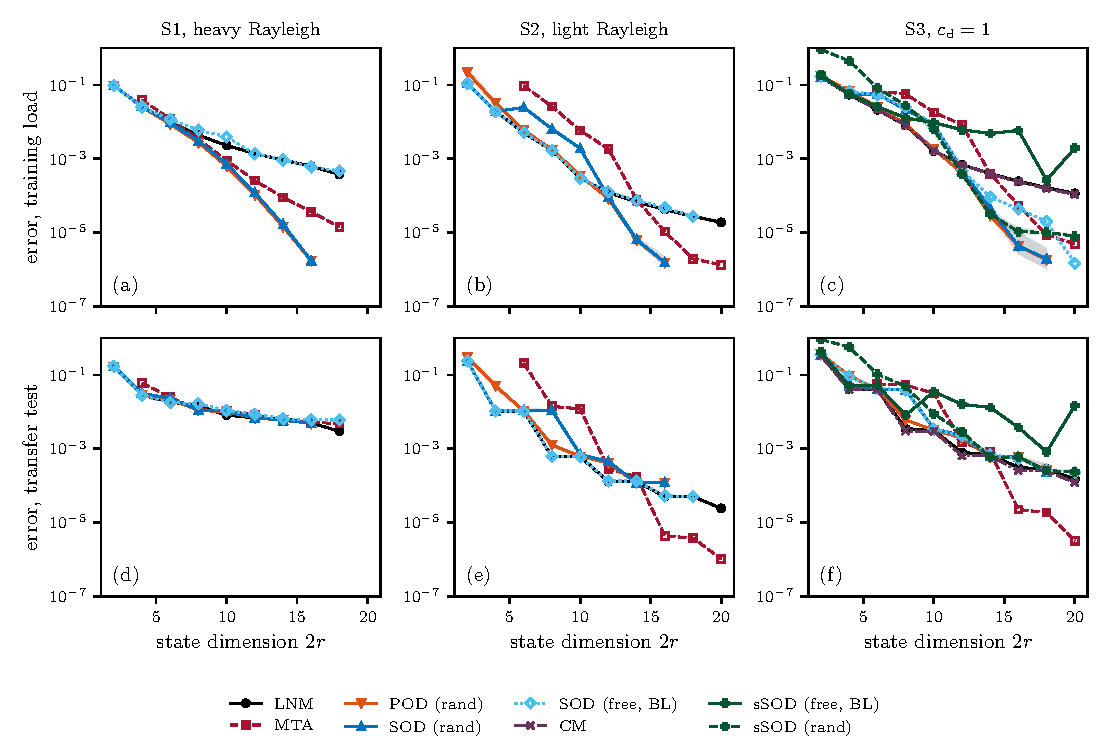
\includegraphics[width=\textwidth]{fig_c_error.pdf}
\caption{ROM displacement error against state dimension $2r$, median and interquartile range over 20 realizations. Columns: S1 with heavy Rayleigh damping; S2 with light Rayleigh damping; S3 with $c_{\mathrm d}=1$. Top: new random load at the training location. Bottom: transfer test (free decay from a floor-4 point load for S1; random mid-span load for S2 and S3). Training signal in brackets; free, BL: order-matched band-limited decay; sSOD: state-space SOD; CM: complex-mode truncation.}
\label{fig:error}
\end{figure}
So the same random-trained basis is worse than the LNMs at intermediate order and better at high order, and the gain belongs to the training load. Sections~\ref{sec:adds} and \ref{sec:displace} explain both.



\section{What the record adds}\label{sec:adds}
Is the high-order gain of a random-trained SOD basis the static correction, and does it serve only the loads the record saw?
We answer first by the geometry of the basis and then by moving the load.

\paragraph{Containment of the static vectors.} Figure~\ref{fig:static}a gives the containment residual \eqref{eq:contain} of the two static load vectors of S2, $\bK^{-1}\bm{b}_{\mathrm{tip}}$ and $\bK^{-1}\bm{b}_{\mathrm{mid}}$, with light damping and the 20 random tip records of Section~\ref{sec:acc}.
\begin{itemize}
\item At $r=8$ the SOD subspace holds the tip vector to $\rho=1.8\times10^{-7}$ (median), against $3.3\times10^{-5}$ for the LNMs, about 190 times closer. At $r=7$ the figures are $1.6\times10^{-6}$ and $5.2\times10^{-5}$.
\item It holds the mid-span vector no better than the LNMs: $7.9\times10^{-5}$ against $3.7\times10^{-5}$ at $r=8$. The record never saw that load.
\item The SOD basis of the order-matched band-limited decay contains no static correction. Its residuals equal those of the LNMs within 12\,\% ($3.6\times10^{-5}$ for the tip vector at $r=8$), as its LNM-level errors in Figure~\ref{fig:error} require.
\end{itemize}
POD of the same records contained the tip vector equally well ($1.7\times10^{-7}$ at $r=8$). At the data rank the two span one subspace.

\paragraph{Principal angles.} At $r=8$, seven of the eight principal angles between the SOD subspace and MTA with the tip vector only were below $0.03^\circ$ (medians); the eighth was $13^\circ$ (at most $15^\circ$). Against the eight LNMs, six angles were below $0.01^\circ$, then $2^\circ$ and $50^\circ$. Against MTA with both static vectors, the largest angle was $69^\circ$, because the mid-span vector is missing.
The random record thus supplies the LNMs it excites and, in place of LNM~8, the static correction of the load it saw.

\begin{figure}[tbp]
\centering
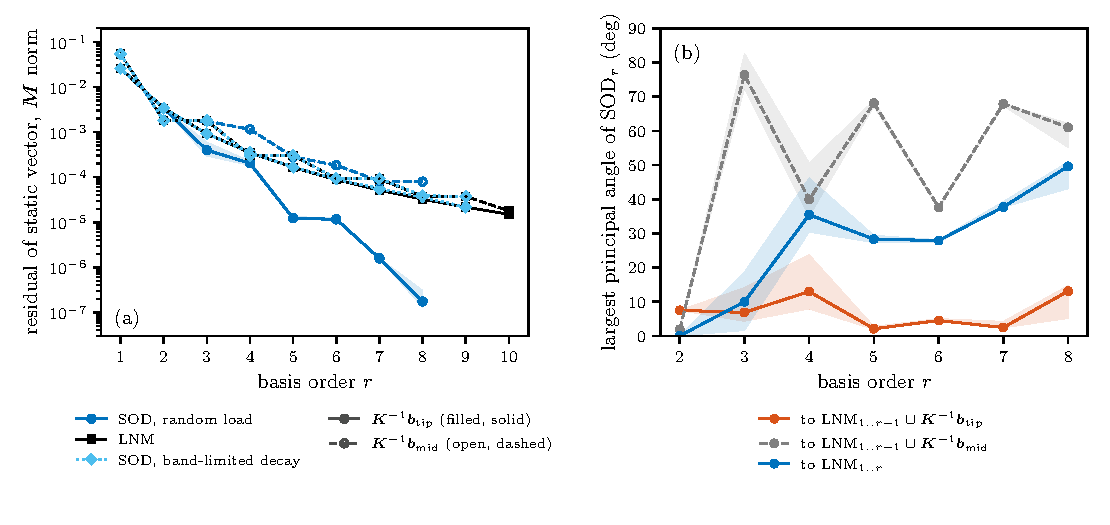
\includegraphics[width=\textwidth]{fig_c_static.pdf}
\caption{What a random tip record adds to the SOD basis; S2, light Rayleigh damping, 20 realizations. (a) Containment residual \eqref{eq:contain} of the static load vectors $\bK^{-1}\bm{b}_{\mathrm{tip}}$ (filled, solid) and $\bK^{-1}\bm{b}_{\mathrm{mid}}$ (open, dashed) against the basis order $r$: SOD of the random tip records (median and interquartile range), LNMs, and SOD of the order-matched band-limited decay. (b) Largest principal angle ($\bM$ metric) between the first $r$ SOD directions and the first $r$ LNMs, and between them and the first $r-1$ LNMs augmented by one static vector; median and range. Scripts: \texttt{g1\_static\_containment.py}, \texttt{g3\_third\_direction.py}, \texttt{mkfig\_c\_static.py}.}
\label{fig:static}
\end{figure}

\paragraph{Transfer: the gain stays at the load locations each basis was given.} For a random load at mid-span, the bases trained at the tip lost their advantage. MTA as defined above contains the static vector of the mid-span load. We therefore also built MTA with the tip vector only. We also trained data bases on independent random loads at both locations. At $r=8$ on the mid-span test:
\begin{itemize}
\item tip only: SOD erred by $1.2\times10^{-4}$ (S2, light) and $3.1\times10^{-4}$ (S2, heavy). MTA with the tip vector erred by $1.1\times10^{-4}$ and $2.9\times10^{-4}$, and the LNMs by $4.8\times10^{-5}$ and $1.4\times10^{-4}$;
\item both locations: SOD erred by $6.0\times10^{-6}$ and $9.0\times10^{-6}$; MTA by $4.2\times10^{-6}$ and $7.9\times10^{-6}$.
\end{itemize}
On S3 the pattern held. SOD and MTA from one location erred by $2.7$--$6.0\times10^{-4}$. From both locations, MTA erred by $1.0$--$2.3\times10^{-5}$ and SOD by $1.9$--$7.8\times10^{-5}$.
So on S2 and S3, SOD and MTA gained at the same load locations: those each basis was given. SOD needs response records at those locations.
On S2 at $r=7$, SOD and LNM were within 10\,\% of each other. The LNM curve for the mid-span load is a staircase, flat at $r=3$, 5 and 7. Mid-span lies within 2\,\% of a node of modes 3, 5 and 7.
On S1 the transfer test, a free decay from a point load at floor 4, was nearly basis-independent. All bases stayed within a factor of 2.1 of one another for $r=3$--9. None was consistently best.
MTA is not uniformly better. On the S2 free-decay test it was 44 times worse than the LNMs at $r=3$. At $r=8$ it was about twice as poor. On S1 it did not beat the LNMs on the floor-4 decay.
The data-driven gain is the persistence problem of \citet{Ilbeigi2017}, seen in a linear system: on S2 and S3 the data bases gained only at the load locations of their records.

\paragraph{Noisy training records.} The gain above used model kinematics. We repeated S2 with measured training records. All 60 displacements carried white noise at 60 or 40\,dB and were smoothed by Whittaker smoothing (WH; penalty on the third difference, 100\,Hz corner, one setting for all channels) \citep{Eilers2003}. Velocities came from the smoothed record (5 realizations).
\begin{itemize}
\item Noise removed the data rank, so the bases reached every order. Their error, however, stopped falling at $r=6$--7.
\item At $r=8$ on the training load, SOD erred by $1.4\times10^{-4}$ (light) and $2.5\times10^{-5}$ (heavy) at 60\,dB. At 40\,dB it erred by $1.4\times10^{-2}$ and $1.5\times10^{-3}$. With model kinematics it erred by $1.5\times10^{-6}$ and $2.0\times10^{-7}$.
\item At 60\,dB SOD was 3 times worse than the LNMs (light) or 5 times better (heavy). At 40\,dB it was 11--300 times worse. POD behaved the same.
\end{itemize}
The floor rose 100-fold for a 10-fold rise in noise amplitude. The high-order gain therefore needs clean training records. For model reduction they should come from the model.
With noise-free training kinematics, the SOD subspace therefore contains the static vector of the training load ($\rho=1.8\times10^{-7}$ at $r=8$, 190 times closer than the LNMs) and not that of the unseen load. MTA adds the same vector from the model.



\section{Why low orders fail}\label{sec:displace}
Why is the random-trained basis worse than the LNMs at $r=3$--5, when it holds the useful direction?
Figure~\ref{fig:static}b and the LNM content of each SOD subspace answer it.

\paragraph{One direction, ranked too early.} The SOD subspace of order $r$ held only $r-1$ LNMs for $r=3$--7 (median $\bM$-residual of each LNM below 0.1). At $r=3$ it held modes 1 and 2; LNM~3 had residual 0.17. At $r=5$ it held modes 1--4, and at $r=6$ modes 1--5, all the modes inside the load band.
The extra direction is the tip static correction. From $r=3$ on, the SOD subspace lay within $2$--$13^\circ$ (medians) of the first $r-1$ LNMs augmented by $\bK^{-1}\bm{b}_{\mathrm{tip}}$. It lay $10$--$50^\circ$ from the first $r$ LNMs, and $38$--$76^\circ$ from the first $r-1$ LNMs augmented by the mid-span vector (Figure~\ref{fig:static}b).
The direction enters at $r=3$ because it is smoother than the upper in-band modes: the third SOD frequency of a random record was 47.7, between modes 2 and 3 (Section~\ref{sec:mix}).
The errors follow the count of in-band modes. Against the LNM ROM the SOD ROM was 4.8 times worse at $r=3$ and 6.5 times worse at $r=5$, while it lacked one in-band mode. At $r=6$, with all five in-band modes present, it was 1.4 times better. At $r=7$ and 8 it was 11 and 27 times better.
The direction that carries the gain at high order is the one that causes the loss at low order.

\subsection{Mixing by training signal}\label{sec:mix}
The same ranking explains how the training signal shapes the basis.
Figure~\ref{fig:mac} compares configuration SOD modes with LNMs by the mass-weighted modal assurance criterion (MAC; \citealp{Allemang2003}; one realization).
\begin{itemize}
\item \emph{Free decay, proportional damping.} On S2, SOD modes 1--8 matched LNMs 1--8 with MAC $\ge0.93$. Frequencies of modes 1--6 were within 0.03--1.6\,\%. The modal coordinates were nearly uncorrelated (largest correlation 0.07).
\item \emph{Random and swept sine.} Extra smooth directions appeared between genuine modes. On S2 with random data, SOD returned frequencies 3.5, 22.0, 47.7, 62.2, 121, 200. The third is a mixture of LNMs 1--3 (MAC 0.19, 0.28, 0.51): the quasi-static tip direction of Section~\ref{sec:displace}. The sweep inserted a direction at 17.1, below mode 2.
\item \emph{Free decay with the dashpot.} Non-proportional damping correlates the modal coordinates (0.71). Configuration SOD modes 2--4 mixed (MAC 0.82, 0.86, 0.58), as the exactness criterion predicts.
\end{itemize}
Every direction ranked among the modes shifts the genuine modes down one rank. A truncated basis then omits a mode it needs, which explains the intermediate-order errors.

State-space SOD on S3 behaves in the same way, plane by plane. From the free decay at $c_{\mathrm d}=0.2$, the pairs 1--2, 3--4, 5--6 and 7--8 matched modal planes 1--4. Their geometric-mean frequencies were within 0.2--2\,\% of $|s_i|$, and the planes within $0.3$--$14^\circ$ in the energy metric. The inter-plane correlation of that decay was 0.14.
At $c_{\mathrm d}=1$ the correlation rose to 0.31, and plane 2 was off by $48^\circ$.
From random or swept-sine records, the smoothest state direction was not modal, and pairs mixed planes, as in configuration space.

\begin{figure}[tbp]
\centering
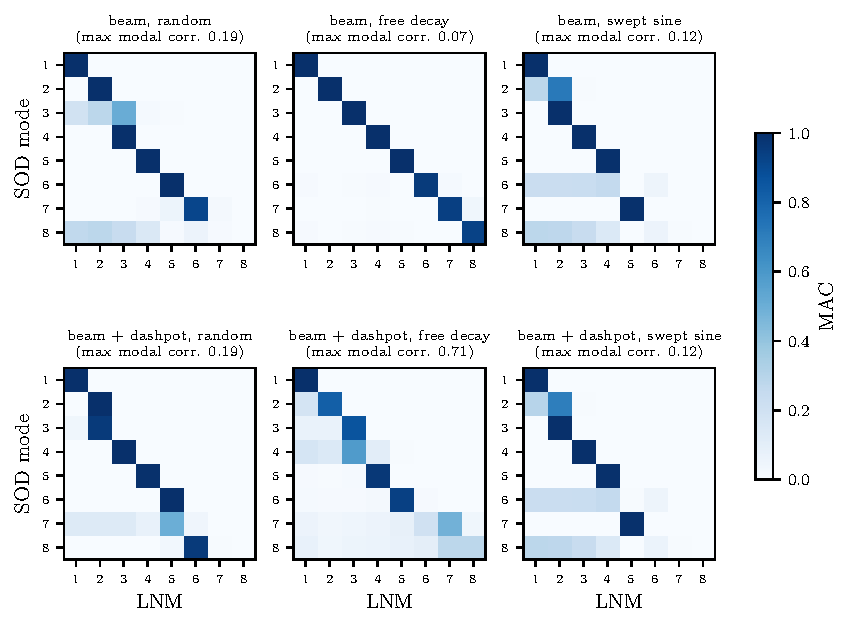
\includegraphics[width=0.92\textwidth]{fig_c_mac.pdf}
\caption{MAC between configuration SOD modes 1--8 (rows, smoothest first) and LNMs 1--8 (columns); the training data excite no higher modes. Top: S2, light damping. Bottom: S3, $c_{\mathrm d}=0.2$. Columns: training signal.}
\label{fig:mac}
\end{figure}

\subsection{Sensitivity to the retained rank}\label{sec:rank}
Smaller rank tolerances admit a second kind of smooth non-modal direction: weakly excited ones. They depend on how much of the near-null data space is kept.
For S2 under a random tip load, POD eigenvalues fall from 1 to $1.7\times10^{-9}$ over eight directions. They then drop to $9\times10^{-12}$ and below.
\begin{itemize}
\item tolerance $10^{-6}$ (rank 6): modes 1--4 clean, mode 5 mixed;
\item tolerance $10^{-10}$ (rank 8): a spurious direction at 46.5 between modes 2 and 3;
\item tolerance $10^{-12}$--$10^{-14}$ (rank 10--11): spurious directions at 1.0--1.7, smoother than mode 1.
\end{itemize}
The spurious directions carried energy fractions of $6\times10^{-5}$--$3\times10^{-4}$, comparable to the fourth and fifth LNM components. An energy threshold therefore cannot separate them.
Weakly excited directions can look smooth. Their mean-square frequency is set by how little they move, not by a mode.
We observed them in clean, band-limited records. Section~\ref{sec:noise} shows how to recognise the genuine modes.
A free decay under proportional damping avoids the displacement, because it contains no quasi-static response. A forced record contains it, and ranking by smoothness misplaces it.


\section{Removing the loss: recognising modes}\label{sec:noise}
How can the quasi-static direction be kept without letting it displace a mode?
For model reduction the kinematics come from the model: velocities and state derivatives are exact, and no measurement noise enters.
Modes are therefore recognised, paired and ordered by their own frequency or circularity, never by their SOD value. Smoothness says how slowly a projection moves. It does not say which mode the projection belongs to, as Sections~\ref{sec:displace} and \ref{sec:rank} show.

\subsection{Recognising modes}\label{sec:recog}
\paragraph{Configuration SOD: spectral consistency.} A coordinate that is a single real mode has its mean-square frequency at its spectral peak. A mixture of modes does not. We read each coordinate's spectrum from its periodogram of the type-II discrete cosine transform (DCT-II), smoothed over $\pm2\,\%$ in frequency. A raw periodogram of a randomly forced coordinate has single-bin spikes. Its arg-max is then not the resonance, and its bin-level width misses the damping width $2\zeta\omega$. Coordinate $i$ is kept if its peak lies within $\max(5\,\%,\,w_i)$ of its SOD frequency $\sqrt{\mu_i}$. Here $w_i$ is the relative half-power width of that peak, capped at 15\,\%. The width makes the test damping-aware. The cap matters. A drifting or broadband coordinate peaks near zero frequency, with a width above 1, and would otherwise pass. The test assumes one frequency per coordinate. A nonlinear decay sweeps that frequency, and the test can then reject a genuine NNM (Section~\ref{sec:nlbb}). Circularity needs no fixed frequency. Two kept coordinates that share one peak cannot both be that mode. The one carrying more response energy, $\|\bphi_i\|^2\avg{q_i^2}$, is kept. Recognised modes are ordered by peak frequency.
We applied a fixed 5\,\% version of this test to the ten smoothest coordinates of clean S2 records. Kinematics came from the model. The test rejected 108 of 134 spurious directions and no genuine mode (10 realizations, tolerances $10^{-10}$--$10^{-14}$). A two-halves rule rejected 102 and also 10 of 147 genuine modes; a lag-diagonality rule rejected 40 and 13.

\paragraph{State SOD: circularity.} Consider the two coordinates of a modal plane. Up to a real change of basis, they are the real and imaginary parts of one complex modal coordinate. SOD returns them uncorrelated and with unit variance, so in their own plane the cloud is round. Read as $z=q_a+\mathrm i\,q_b$, the pair rotates one way and the spectrum of $z$ is one-sided. Two unrelated coordinates, or coordinates of two different planes, give a nearly symmetric spectrum.
Pairs are therefore formed by matching, not by rank. Candidate pairs are paired greedily by one-sidedness and kept above 0.85; only one plane is kept per frequency. A loose frequency gate, four times the spectral tolerance, only limits the search. The plane frequency is the peak of the one-sided spectrum of $z$, and planes are ordered by it.
Pairing by rank fails. Pairing adjacent coordinates in SOD order lost the slowest plane of random-load records, because a quasi-static coordinate sat between its two members. Requiring the two members' raw spectral peaks to agree lost it in 4 of 10 records, because those peaks scattered by up to 21\,\% under random forcing. With smoothed spectra and the loose gate, the mode-1 plane was recognised in all 8 test records. Modal planes gave a one-sidedness of 0.89--0.99, other pairs 0.51--0.75. A strong plane can be contaminated by another mode at its own frequency, which lowers its one-sidedness. A pair scoring 0.75--0.85 is therefore also kept under two conditions. Its one-sidedness within $\pm30\,\%$ of its peak must be at least 0.95. It must also carry at least 1\,\% of the response energy. The banded test alone is unsafe. On noisy linear records it admitted up to 15 times more non-modal pairs. Two narrowband noise coordinates in quadrature also look circular. With the energy gate, the model-reduction results did not change. From one random-load record on S3 ($c_{\mathrm d}=0.2$) the recognised planes were at 3.7, 22.1, 62.5, 121.2 and 201.4\,rad/s. From the band-limited decay they were at 3.5, 22.0, 61.7, 120.9 and 199.6\,rad/s. The damped frequencies are 3.5, 22.0, 61.7, 120.9 and 199.7\,rad/s.

\subsection{Selection for model reduction}\label{sec:romsel}
We compared four bases from the same SOD, with model kinematics (10 realizations):
\begin{itemize}
\item R0: the plain basis, in SOD order;
\item RID: the recognised modes or planes only, up to $1.2\,\omega_{\mathrm c}$, ordered by frequency;
\item RH: the recognised modes first, by frequency, then the remaining coordinates in SOD order;
\item RHB: as RH, but only recognised modes inside the load band, $\omega\le\omega_{\mathrm c}$, go first.
\end{itemize}
Modes above the load band respond quasi-statically to it. The smooth direction that carries that response serves a ROM better than the mode itself. This is why RHB stops at $\omega_{\mathrm c}$.
\paragraph{S2, random tip load.} RHB removed the low-order damage of spurious directions. In no record was it more than 11\,\% worse than R0 at any order.
\begin{itemize}
\item Tolerance $10^{-12}$: the median two-mode error fell from $1.1\times10^{-1}$ to $2.0\times10^{-2}$ on the training load. At mid-span it fell from $2.2\times10^{-1}$ to $1.0\times10^{-2}$. The four-mode errors fell from $6.1\times10^{-3}$ to $1.8\times10^{-3}$ and from $1.0\times10^{-2}$ to $6.5\times10^{-4}$.
\item Tolerance $10^{-10}$: the four-mode mid-span error fell from $1.1\times10^{-2}$ to $7.6\times10^{-4}$.
\item At $r=6$ RHB equalled R0 at tolerance $10^{-10}$ and improved it at $10^{-12}$ ($1.7\times10^{-4}$ to $1.0\times10^{-4}$ on the training load). At $r=8$ all bases erred by $1.4\times10^{-6}$ on the training load.
\end{itemize}
RH also puts the recognised mode 6 (about 295\,rad/s) first. It was 1.3--10 times worse than R0 on the training load at $r=6$ and tolerance $10^{-10}$, though better at mid-span. RID alone stops at the six modes below $1.2\,\omega_{\mathrm c}$.
\paragraph{S3, $c_{\mathrm d}=0.2$, state SOD.} From random-load records RHB improved state dimension 4 in every record (median training-load error $2.9\times10^{-1}\to1.0\times10^{-1}$, mid-span $3.7\times10^{-1}\to9.2\times10^{-2}$). At state dimension 8 it was slightly worse (median ratio 1.1--1.2, at most 2.5 in one record). From 12 on it equalled R0. Planes from forced records are tilted by their quasi-static response (Section~\ref{sec:ic}). From the band-limited decay the recognised order matched the SOD order, and all bases were identical.
\paragraph{Can a frequency place the other coordinates?} Two further orders placed every coordinate by a frequency.
\begin{itemize}
\item RF: recognised modes at their peak frequency, all other coordinates at their SOD frequency $\sqrt{\mu}$.
\item RQ: every coordinate at the Rayleigh-quotient frequency of its displacement shape, $\sqrt{\bphi^{\mathsf T}\bK\bphi/\bphi^{\mathsf T}\bM\bphi}$, from the model. For state SOD both members of a plane take the geometric mean of their two values.
\end{itemize}
RF gave the same ROMs as R0 in every record (S2 at both tolerances, S3 at $10^{-10}$). The SOD frequency of a quasi-static direction follows the load spectrum, not the structure. Here it never moved past a mode.
RQ was no better than R0 at $r=6$ and 8 on S2. The median ratio was 1.0--4.0 at tolerance $10^{-10}$ and 1.0--57 at $10^{-12}$. On S3 it was worse from state dimension 12. The median ratio was 1.3--220 on random records; the ratio was 2.3--5.5 on the single band-limited decay.
At tolerance $10^{-12}$ it improved $r=2$ (median ratio 0.5--0.6), but RHB did as well or better. A quasi-static direction is stiff, so RQ moves it to the end of the basis. A ROM of low order then cannot use it.
The value of such a direction lies in its share of the forced response. The SOD order already measures that share.
For model reduction we therefore recommend RHB. Recognised in-band modes come first, by frequency; the rest follow in SOD order.
Recognition thus keeps the static-correction direction in the basis but places it behind the in-band modes it displaced.


\section{Complex modes}\label{sec:complex}
Does the picture survive non-proportional damping, where the modes are complex and configuration SOD cannot represent them?
\paragraph{Complex modes: state-space SOD restores much of the modal basis.} On S3 the modes are complex. Configuration SOD from free decay mixed the modes; state-space SOD mixed them much less.
On the forced tests, complex modes bought little. A configuration ROM was built on the undamped LNMs, with the full damping matrix projected. It erred within 25\,\% of complex-mode truncation at every order (ratio 0.96--1.25). On the free test decay complex-mode truncation was 2.5--7 times better at state dimension 8. Configuration SOD fails on S3 because its modes mix, not because the true modes are complex.
At state dimension 8, with BL training (SR in brackets; Section~\ref{sec:ic} compares other decays):
\begin{itemize}
\item $c_{\mathrm d}=0.2$: state SOD erred by $4.6\times10^{-3}$ ($4.5\times10^{-3}$), $2.0\times10^{-3}$ ($2.1\times10^{-3}$) and $9.8\times10^{-4}$ ($2.2\times10^{-4}$) on the random, mid-span and SR-decay tests. Configuration SOD erred by $1.7\times10^{-2}$, $2.7\times10^{-2}$ and $6.5\times10^{-4}$, and complex-mode truncation by $4.3\times10^{-3}$, $1.5\times10^{-3}$ and $4.3\times10^{-5}$;
\item $c_{\mathrm d}=1$: state SOD $1.3\times10^{-2}$ ($9.0\times10^{-3}$), $8.0\times10^{-3}$ ($6.8\times10^{-3}$), $3.9\times10^{-3}$ ($5.9\times10^{-4}$); configuration SOD $2.5\times10^{-2}$, $3.9\times10^{-2}$, $7.7\times10^{-4}$; complex-mode truncation $8.2\times10^{-3}$, $3.0\times10^{-3}$, $5.6\times10^{-5}$.
\end{itemize}
Consider forced tests at state dimension 8. State SOD from the BL decay came within a factor of 2.7 of complex modes. At 10--16 the factor grew to 1.9--25. It was also within that factor of the LNM ROM (1.1--2.3). It cut the mid-span error of configuration SOD by 5--13 times (random tip test: 2--4). On the SR-decay test it stayed 20--70 times above the complex modes (SR training: 5--10 times). The planes are estimated from a short, correlated decay, and part of this gap is the initial-state projection (Section~\ref{sec:ic}).
Above state dimension 8 the BL state SOD error stalled near $10^{-3}$ on the random test. The SR basis kept improving, to $6.9\times10^{-5}$ at state dimension 16 for $c_{\mathrm d}=0.2$. Its error stopped falling above 14--16. On the mid-span test it rose already from 10 to 12, and at $c_{\mathrm d}=1$ it became erratic. Weakly excited planes are poorly determined by a decay.
State SOD from forced records was poor at low order: $6.1\times10^{-1}$ at state dimension 2 for $c_{\mathrm d}=0.2$. Its smoothest directions are forced, not modal (Section~\ref{sec:mix}).
No energy-Galerkin state ROM was unstable.

\paragraph{Trajectories.} Figure~\ref{fig:traj} compares tip responses at state dimension 8 for one realization (seed 2026).
On S2 under the mid-span load, the LNM ROM overlays the full model. So does the SOD ROM from the equal-energy decay. Their errors were $5.7\times10^{-4}$ and $5.9\times10^{-4}$. Random-trained SOD and MTA erred by $1.0\times10^{-2}$ and $1.3\times10^{-2}$; at $r=4$ MTA keeps only two LNMs.
On S3 with $c_{\mathrm d}=1$, complex-mode truncation erred by $2.9\times10^{-3}$. State SOD from the static-release and band-limited decays erred by $6.6\times10^{-3}$ and $8.1\times10^{-3}$. State SOD from the equal-energy decay drifted visibly, $1.2\times10^{-1}$ (Section~\ref{sec:ic}).

\begin{figure}[tbp]
\centering
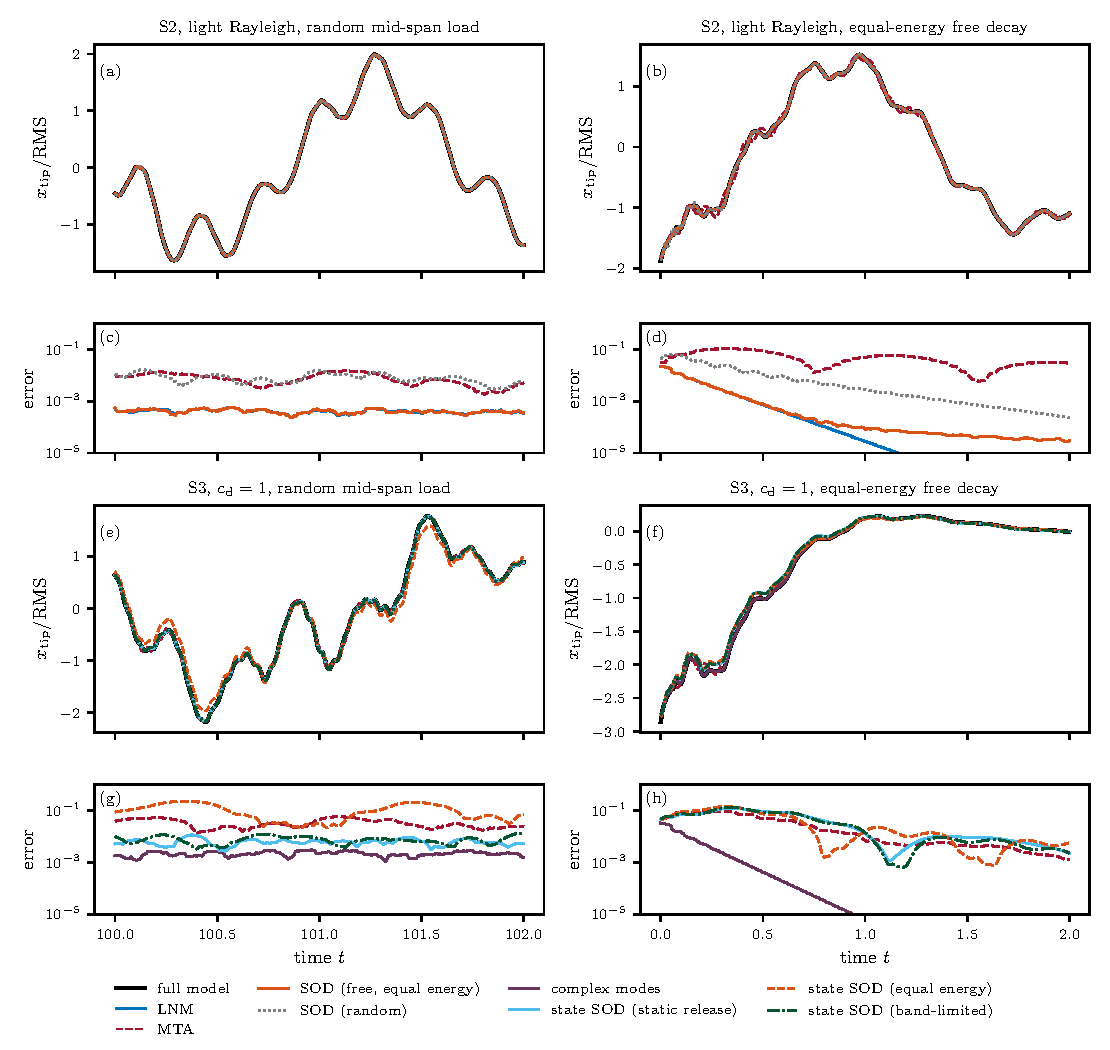
\includegraphics[width=\textwidth]{fig_c_traj.pdf}
\caption{Tip displacement of the full model and ROMs at state dimension 8, one realization. Left: random mid-span load, $t=100$--102. Right: equal-energy test decay ($b_k=(-1)^{k-1}$). (a,b) S2, light Rayleigh damping, configuration ROMs (SOD from the equal-energy decay and from a random tip load). (e,f) S3, $c_{\mathrm d}=1$, state ROMs, MTA and complex modes. (c,d,g,h) Error: root-mean-square (RMS) value of the tip-displacement difference over a sliding 0.1 window. It is divided by the RMS of the full-model tip displacement over the plotted window. Training decays for state SOD: static release, equal energy, and band-limited with $\omega_{\mathrm b}=\omega_4$.}
\label{fig:traj}
\end{figure}

\subsection{Which free decay to train on}\label{sec:ic}
Impact testing aims to excite every mode in the band of interest, with similar force at each frequency. The hammer tip sets that band: a hard tip widens it, a soft tip narrows it. An equal-energy initial state is the numerical analogue of a hard tip. We therefore repeated the free-decay training with EE and BL decays, one realization per case and the ensemble seeds.
Random-trained bases do not depend on the initial state; the random tests reproduce the first ensemble realization.
Away from the data rank, ensemble scatter reached 0.76 of the median. Single-realization differences below a factor of two are therefore not significant.
Figure~\ref{fig:ic} shows the results. For the BL and SR bases, these values agree with the 20-realization medians of Section~\ref{sec:acc} within a factor of 1.25.

\paragraph{Configuration SOD.} Under light Rayleigh damping the initial state hardly mattered on S1 and S2. EE, BL and SR errors agreed within a factor of 1.3 up to $r=5$, and within 2.5 above.
Under heavy Rayleigh damping two effects competed (Figure~\ref{fig:ic}c,d).
\begin{itemize}
\item \emph{Rank.} The static-release decay ended at the data rank: $r=7$ on S1, 6 on S2. EE and BL decays with $\omega_{\mathrm b}=\omega_r$ reached $r=9$ on S2 and the full order on S1.
\item \emph{Accuracy.} At $r=3$--6, EE was 1.3--2.6 times worse than SR on S2 and 2.9--14 times worse on S1. On S1 at $r=4$ it erred by $1.1\times10^{-2}$ against $2.8\times10^{-3}$, and BL with $\omega_{\mathrm b}=\omega_r$ by $5.8\times10^{-3}$.
\end{itemize}
On S3, EE helped configuration SOD at low order. With $c_{\mathrm d}=1$ and the random tip load, it matched complex-mode truncation at $r=2$--4 ($8.1\times10^{-3}$ at $r=4$). The SR basis erred by $2.0\times10^{-2}$.

\paragraph{State-space SOD.} Equal excitation of all modes hurt the state ROMs (Figure~\ref{fig:ic}e,f).
At state dimension 8 and the mid-span load, EE gave $1.3\times10^{-2}$ ($c_{\mathrm d}=0.2$) and $1.2\times10^{-1}$ ($c_{\mathrm d}=1$). SR gave $2.0\times10^{-3}$ and $6.7\times10^{-3}$; complex-mode truncation $1.5\times10^{-3}$ and $3.0\times10^{-3}$.
Band-limiting at $\omega_{\mathrm b}=\omega_r$ restored SR accuracy on forced tests at state dimension 8 and below, within a factor of 1.5. At state dimension 10--16 SR remained best on the random test. At state dimension 12 and $c_{\mathrm d}=1$ it erred by $5.2\times10^{-4}$ on the random test. BL erred by $6.2\times10^{-3}$ and complex modes by $6.7\times10^{-4}$.
Band-limiting at the load cutoff, $\omega_{\mathrm b}=\omega_{\mathrm c}$, still left the state ROMs 2--7 times worse than SR. This held on the forced tests at state dimension 8.

\paragraph{Mechanism.} A transient does not decorrelate the modal planes. Their normalized cross-correlation over a decay from rest depends on damping and frequency spacing, not on record length or amplitude. Its largest value in our records was 0.12 (S2), 0.14 ($c_{\mathrm d}=0.2$) and 0.32--0.34 ($c_{\mathrm d}=1$). It was the same for every initial state that excites modes 1--9.
By Proposition~\ref{prop:ssod}, correlation tilts the smooth planes at first order. The tilt toward a plane outside the ROM grows with that plane's share of the record energy.
We measured the energy-norm leakage of the eight-state SOD subspace out of modal planes 1--4. It was $5.5\times10^{-2}$ (SR), $1.0\times10^{-1}$ (EE) and $2.5\times10^{-1}$ (EE weighted to equal record energy) on S2.
When the leakage exceeded 0.05, the Galerkin ROM converted it into a relative eigenvalue error (Figure~\ref{fig:ic}b). The error was 0.2--0.8 times the leakage squared. At $c_{\mathrm d}=1$, decays with leakage below 0.04 left a floor of $3\times10^{-4}$--$6\times10^{-3}$. With light damping a small frequency error becomes a large response error near resonance. Equal record energy raised the S2 error to $1.7\times10^{-1}$.
The rule for clean data is therefore not equal excitation. It is little energy above the retained band, relative to the energy inside it. Static release meets it because its modal energy falls steeply with mode number (Figure~\ref{fig:ic}a).
Equal excitation helps where rank is scarce: heavy damping, or noise that buries weakly excited modes. Matching the excited band to the ROM order serves both. A hammer tip is matched to the band of interest in the same way.

\paragraph{Free-decay tests of state ROMs.} On the EE test decay, every state SOD ROM erred by $2$--$6\times10^{-2}$ at state dimension 8. This held whether it was trained on the SR, EE or BL decay. Complex modes erred by $5$--$6\times10^{-3}$ (Figure~\ref{fig:traj}h). The cause is the initial state, not the basis. Energy-orthogonal projection maps truncated planes onto retained ones when the modes are complex. Projection with the data covectors was worse, $2.4$--$2.5\times10^{-1}$. Complex-mode truncation uses the exact left eigenvectors.

\begin{figure}[tbp]
\centering
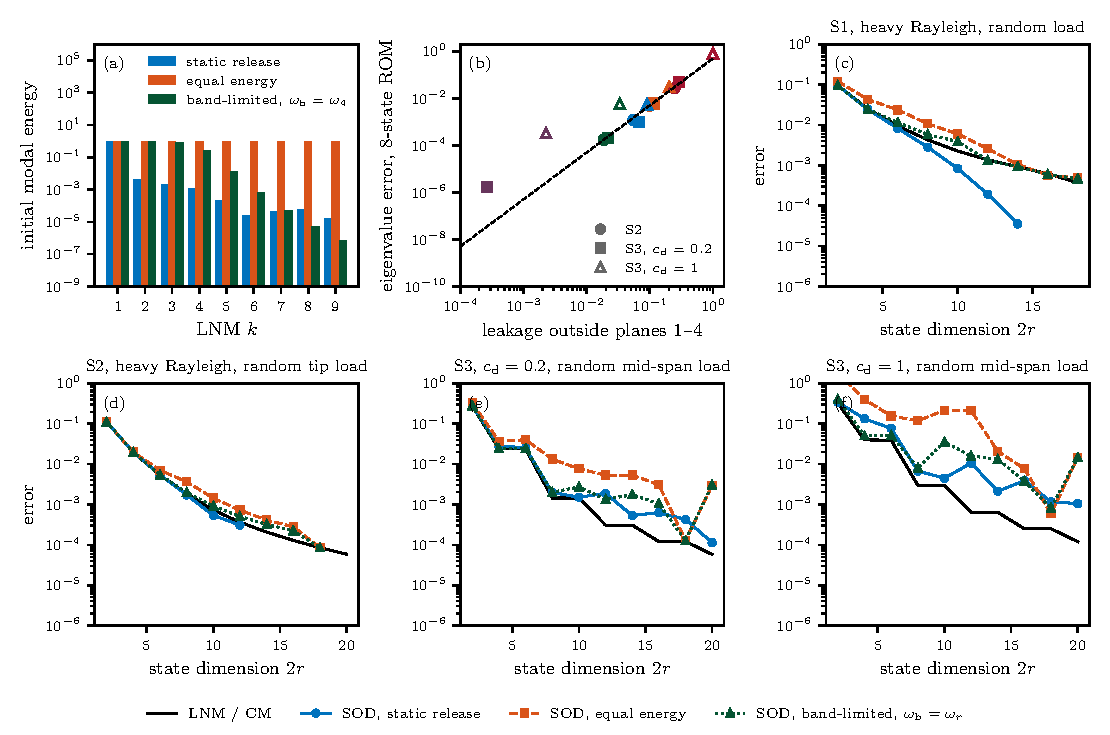
\includegraphics[width=\textwidth]{fig_c_ic.pdf}
\caption{Choice of training decay, one realization. (a) Initial modal energy on the cantilever: static release, equal energy over modes 1--9, and band-limited equal energy with $\omega_{\mathrm b}=\omega_4$. (b) Leakage of the eight-state state-SOD subspace out of modal planes 1--4. It is plotted against the largest relative eigenvalue error of its energy-Galerkin ROM. All training decays are shown (colours as in a; red: equal record energy; plum: modes 1--4 only). Dashed: $0.5\times$ leakage squared. (c,d) Configuration SOD, heavy Rayleigh damping, new random load at the training input. (e,f) State-space SOD on S3, random mid-span load; the solid black line is complex-mode truncation. Band-limited decays use $\omega_{\mathrm b}=\omega_r$.}
\label{fig:ic}
\end{figure}
With complex modes, too, the state-SOD planes follow the record. A decay gives planes tilted toward the modes it excites above the retained band, and a forced record gives planes tilted by its quasi-static response.

\section{Nonlinear benchmarks}\label{sec:nl}
Does the energy dependence of decay data help a nonlinear ROM? We test two nonlinear cantilevers: S4 for backbone accuracy and S5 for forced bifurcations.
Nonlinear ROMs proper reduce onto invariant manifolds: nonlinear normal modes \citep{Shaw1993,Touze2004} and spectral submanifolds \citep{Haller2016,Cenedese2022}. Model-based alternatives augment the modes with static or derivative vectors, or with a quadratic manifold built from them \citep{Idelsohn1985,Jain2017}; \citet{Mignolet2013} review non-intrusive ROMs of geometrically nonlinear structures, including the choice of basis; \citet{Touze2021} review invariant-manifold methods and the quadratic manifold. We do not compete with them. We test linear Galerkin bases only, where SOD is an alternative to LNM, MTA and POD.

\subsection{Backbone accuracy}\label{sec:nlbb}
S4 is the COST F3 cantilever of Section~\ref{sec:bench} (Figure~\ref{fig:systems}d).

\paragraph{Reference backbone.} We computed the NNM1 backbone \citep{Kerschen2009} of the full model by odd harmonic balance \citep{Detroux2015}. It used eight harmonics and pseudo-arclength continuation.
We integrated the full model over one period from the balanced initial state, at four energies. It returned to that state within $1.5\times10^{-10}$ or better.
The backbone rises from 23.66\,Hz to 42.1\,Hz at total energy $H=3\times10^{-2}$\,J.
A 5:1 internal resonance with mode 2 (148.3\,Hz) forms a tongue at 29.9--30.4\,Hz (Figure~\ref{fig:nl}a). The main backbone is interrupted between $H=3.6\times10^{-3}$ and $4.0\times10^{-3}$\,J, where the tongue branches off. The tongue itself stays near 30\,Hz up to the highest energy computed.
There the fifth harmonic exceeds the fundamental. We compare backbones outside the tongue only.
Plucked responses from static deflections are not on the backbone. Their zero-crossing frequencies lay up to 3\,\% below it at the same energy. The plucked state also excites higher modes.

\paragraph{Bases.} LNM; MTA with the static tip-load vector; and SOD and POD of one damped decay ($\zeta=0.01$, Rayleigh on modes 1--2). Two decays were used. The band-limited decay follows the convention of Section~\ref{sec:bench}. It is an equal-energy sum of LNMs 1--4, the band of interest for $r\le4$. The static-release decay starts from the deflection under a 30\,N tip load. The results below are for static release; the band-limited decay follows them. It lasts 1.5\,s and sweeps the energy down the backbone.
Each ROM backbone was computed by the same harmonic balance on the reduced equations.

\paragraph{Results.} Median backbone frequency errors over 24 energies outside the tongue, from $6\times10^{-4}$ to $2.5\times10^{-2}$\,J (Figure~\ref{fig:nl}b):
\begin{itemize}
\item $r=1$: LNM $1.1\times10^{-2}$, SOD and POD $2.2\times10^{-3}$;
\item $r=2$: LNM $1.5\times10^{-3}$, MTA $8\times10^{-5}$, SOD $1.4\times10^{-4}$, POD $2.1\times10^{-4}$;
\item $r=3$: LNM $4.7\times10^{-4}$, MTA $1.4\times10^{-6}$, SOD $2.0\times10^{-6}$, POD $1.2\times10^{-5}$;
\item $r=4$: LNM $2.0\times10^{-4}$, MTA $1.4\times10^{-6}$, SOD $5\times10^{-7}$, POD $4\times10^{-7}$.
\end{itemize}
At $r=3$ and 4, decay-trained bases improved the backbone by two to three decades over the LNMs. At $r=2$ the gain was about one decade. The model-based static tip-load vector did as well or better at $r=2$ and 3, and SOD was better at $r=4$.
Both contain the deformation that the localized cubic force imposes on the beam: MTA as $\bK^{-1}\bm{e}_{\mathrm{tip}}$, SOD in its first direction, $0.3$--$0.9^\circ$ from the shape $(\bK-\omega^2\bM)^{-1}\bm{e}_{\mathrm{tip}}$ forced at the NNM frequency (see below).
SOD led POD at $r=2$ and 3; at $r=4$ POD was 1.4 times better.

\paragraph{Held-out time-domain tests.} Conservative responses started from static deflections not used in training. The loads were 3, 10 and 20\,N at the tip and 20 and 60\,N at mid-span.
At $r=4$, MTA, SOD and POD gave displacement errors of $1.5$--$5.5\times10^{-3}$ over 0.1\,s. The LNMs gave $4.5\times10^{-4}$ to $1.1\times10^{-2}$, better at low energy and worse at high energy. Zero-crossing frequency errors were at most $1.1\times10^{-4}$ for SOD and MTA, and up to $9.1\times10^{-4}$ for the LNMs.
At $r=2$, SOD gave displacement errors of $0.8$--$4.8\times10^{-2}$, MTA $4$--$13\times10^{-2}$.
The plucked states excite modes that a backbone-dominated record does not contain. At $r=4$ displacement accuracy in these tests was therefore limited by the truncated modes: MTA, SOD and POD gave errors within the same range.
Figure~\ref{fig:nltraj} shows two of these tests over 0.3\,s. At $r=4$ the LNM error grows with time, from phase drift. Over the record it was $1.8\times10^{-2}$ (20\,N tip) and $3.3\times10^{-2}$ (60\,N mid-span). The MTA and SOD errors stay flat, $3.6$--$5.6\times10^{-3}$ over the record, set by the truncated modes.

\paragraph{Band-limited training decay.} The band-limited decay starts from an equal-energy sum of LNMs 1--4. Each holds the potential energy of the 30\,N state, $1.48\times10^{-2}$\,J. The total, including the cubic-spring energy, was $8.0\times10^{-2}$\,J.
SOD backbone errors were $5.8\times10^{-3}$, $1.7\times10^{-4}$, $4.9\times10^{-6}$ and $4.1\times10^{-7}$ for $r=1$--4, within a factor of 2.7 of the static-release values. POD was hurt more: $2.8\times10^{-5}$ at $r=4$, against $4\times10^{-7}$.
In the plucked tests the $r=4$ errors were unchanged, $1.6$--$5.5\times10^{-3}$. At $r=2$ they rose to $3.0\times10^{-2}$--$1.1\times10^{-1}$, against $0.8$--$4.8\times10^{-2}$ from static release. As in the linear tests, energy in modes outside a low-order basis costs accuracy.

\paragraph{Tracking the backbone.} Figure~\ref{fig:track}a draws the ROM backbones on the frequency--energy plot. At full scale every two-mode ROM sits on the full-model backbone; all run high as the energy grows. At 0.02\,J the LNM ROM was $5.2\times10^{-3}$ high, MTA and SOD $1.5\times10^{-3}$. At 0.05\,J SOD stayed closest: $3.0\times10^{-3}$, against $6.5\times10^{-3}$ (LNM) and $8.9\times10^{-3}$ (MTA). The four-mode SOD ROM matched to about $10^{-6}$ up to 0.048\,J. There an internal-resonance tongue of the ROM itself begins; the full model's begins at 0.059\,J.
SOD can also read the backbone from the record alone, without a ROM. We slid 0.12\,s windows (3--5 periods) along the static-release decays from 30 and 120\,N. The hop was 0.03\,s.
\begin{itemize}
\item \emph{Configuration SOD:} the frequency of the smoothest coordinate, $\sqrt{\mu_1}/(2\uppi)$.
\item \emph{State SOD:} the NNM1 plane, recognised by circularity, read by the product rule $(\mu_a\mu_b)^{1/4}/(2\uppi)$. NNM1 is taken as the slowest plane whose product-rule frequency agrees with its spectral peak. No reference is used.
\end{itemize}
The state-SOD plane followed the backbone with median errors of $2.6\times10^{-3}$ (30\,N) and $1.2\times10^{-3}$ (120\,N). Its errors were at most $5\times10^{-2}$ (Figure~\ref{fig:track}b,c). Configuration SOD erred by $1.3$--$1.6\times10^{-2}$ in median.
The windows are neither closed nor free of mode 2, which the static release excites strongly. The smoothest configuration coordinate mixes the two. The state plane separates them, because circularity recognises each plane by its own rotation.

\begin{figure}[tbp]
\centering
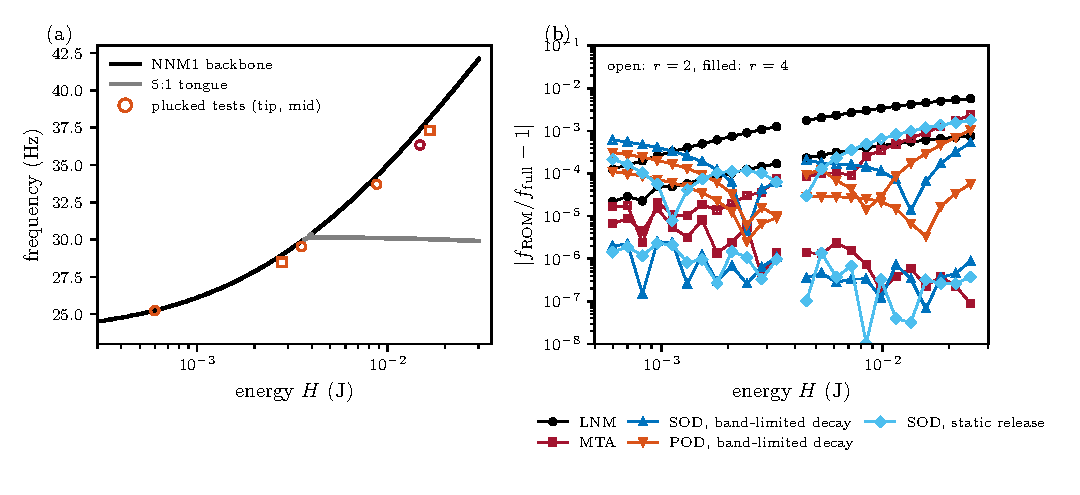
\includegraphics[width=\textwidth]{fig_c_nl.pdf}
\caption{COST F3 cantilever with cubic tip spring. (a) Frequency--energy plot of NNM1 from harmonic balance: main backbone, 5:1 tongue, and zero-crossing frequencies of the plucked tests. Circles: tip loads; squares: mid-span loads; dark: the 30\,N training state. (b) Backbone frequency error of the ROMs against energy, outside the tongue; open: $r=2$, filled: $r=4$. SOD and POD from the band-limited decay (LNMs 1--4, equal energy), and SOD from the static release.}
\label{fig:nl}
\end{figure}

\paragraph{Bending out of the plane.} As the energy rises, the NNM leaves the plane of LNM~1. We applied state SOD to decays released from 30, 60, 120 and 240\,N (initial energies 0.015--0.22\,J). Accelerations came from the equations of motion.
\begin{itemize}
\item Circularity recognised the NNM1 plane in every decay (one-sidedness 0.97--0.99). Spectral consistency on configuration SOD rejected it at 30 and 60\,N. The decay sweeps the NNM frequency, and peak and SOD frequency separated by 10--12\,\%.
\item One non-modal coordinate peaked inside the plane's swept band. Its energy share grew with the load, from $2\times10^{-4}$ to $3.6\times10^{-3}$. With the plane it spans a configuration space $2.1^\circ$ from LNMs 1--2: it is the bend toward mode 2.
\item Band-passed to the swept band, the record had two significant configuration directions, then a drop of 2--3 decades. The state record had four, then a drop by 17--38; the drop after the second value was 4--16. This is consistent with one bend direction, adding one configuration and two state directions. A bent NNM with $\ell$ such directions needs $1+\ell$ configuration and $2+2\ell$ state directions. The bend, and hence $\ell$, depends on amplitude; a decay sweeps through it.
\end{itemize}
At 30\,N the bend also contaminated the mode-2 plane, which then failed the circularity test (0.836). The rescue rule of Section~\ref{sec:recog} recovered it.
We then ordered a configuration basis by frequency. Each recognised plane enters by its dominant displacement direction, followed by the coordinates peaking in its band. The rest follow in SOD order. Against configuration SOD at $r=2$--4, its backbone error was within 3\,\% or better at every load. At $r=3$ and 60\,N it was $1.8\times10^{-6}$ against $3.9\times10^{-6}$, as low as MTA. On motion started on the NNM it was 2--3 times worse at $r=4$ for 120 and 240\,N.
Frequency and circularity therefore recognise the bent NNM and its out-of-plane direction. As an ordering they helped at 60\,N, by 2.2--3.3 times on the backbone at $r=2$ and 3. Otherwise they changed ROM accuracy little. Configuration SOD's first direction already lies $0.3$--$0.9^\circ$ from $(\bK-\omega^2\bM)^{-1}\bm{e}_{\mathrm{tip}}$, the shape forced at the NNM frequency. Here $\bm{e}_{\mathrm{tip}}$ is the unit load at the tip displacement. The same direction lies $1.1$--$2.7^\circ$ from LNM~1.

\begin{figure}[tbp]
\centering
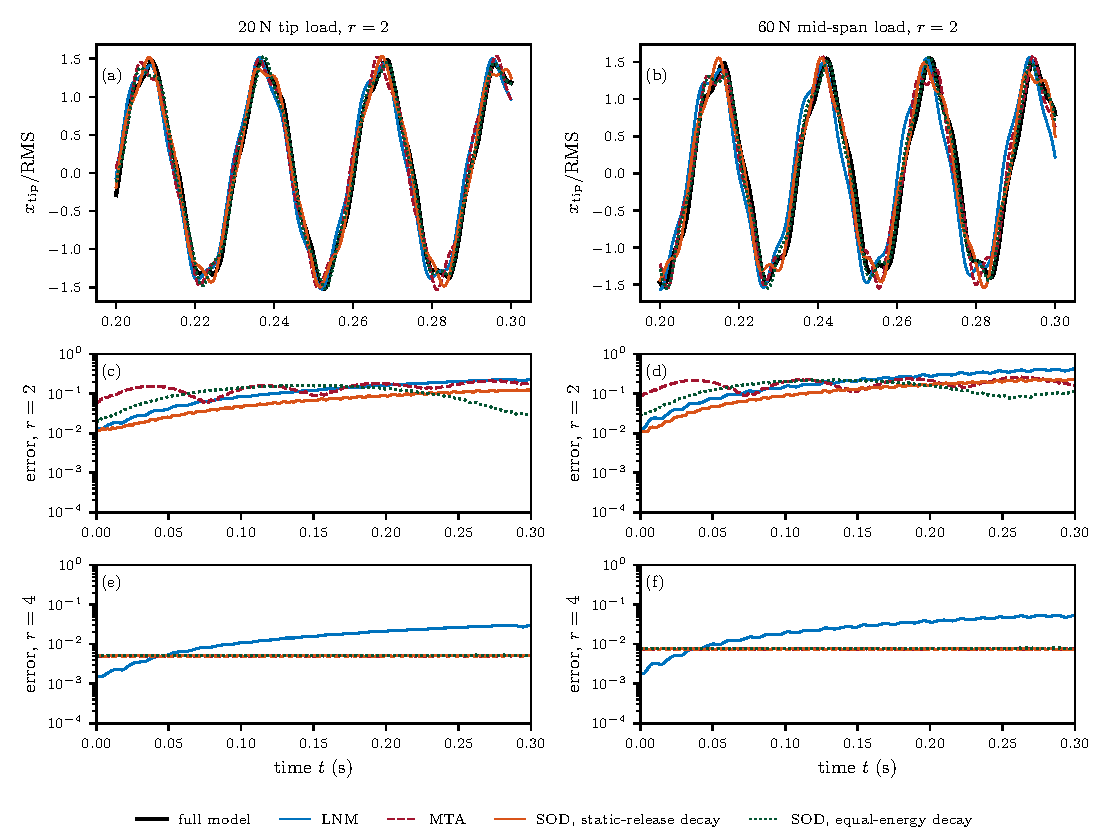
\includegraphics[width=\textwidth]{fig_c_nltraj.pdf}
\caption{COST F3 cantilever, held-out plucked tests released from rest. Static deflection under 20\,N at the tip (left) and 60\,N at mid-span (right). (a,b) Tip displacement of the full model and two-mode ROMs, $t=0.2$--0.3\,s, divided by the RMS full-model tip displacement. (c--f) RMS tip error over a sliding 0.03\,s window (about one period), same normalization: $r=2$ (c,d) and $r=4$ (e,f). SOD bases from the static-release decay (30\,N tip load) and the equal-energy decay (LNMs 1--4).}
\label{fig:nltraj}
\end{figure}

\paragraph{Cost.} All models were integrated by average-acceleration Newmark. At $\Delta t=2\times10^{-5}$\,s the full model took 0.89\,s and the LNM, SOD and POD ROMs 0.45--0.58\,s, best of three (\texttt{n2b\_cost\_best3.py}). The differences among ROMs are within the run-to-run spread of up to 27\,\%. Two- and four-mode ROMs took the same time, so per-step overhead, not model size, set it.
The full model and these ROMs held the tip frequency within $10^{-3}$ at $\Delta t=4\times10^{-4}$\,s. The exception was the two-mode POD ROM, which needed $2\times10^{-4}$\,s.
Central differences need $\Delta t<2/\omega_{\max}$: $2.0\times10^{-6}$\,s for the full model and $3.3$--$3.9\times10^{-4}$\,s at $r=4$.

\begin{figure}[tbp]
\centering
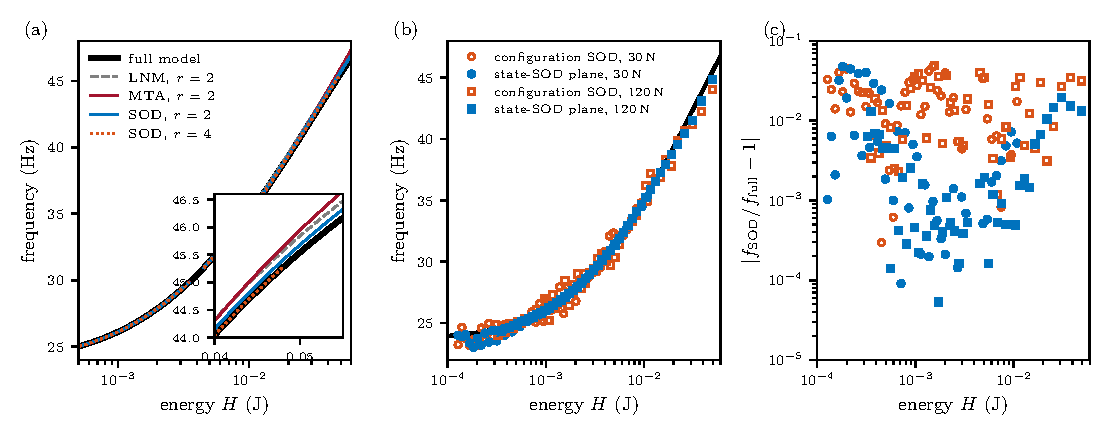
\includegraphics[width=\textwidth]{fig_c_track.pdf}
\caption{COST F3 cantilever (S4): how well SOD follows the NNM1 backbone. (a) Backbones of two-mode ROMs (LNM, MTA, SOD of the 30\,N static-release decay) and of the four-mode SOD ROM. They are drawn on the full-model frequency--energy plot; inset: high-energy end, linear axes. (b) Frequency read from 0.12\,s windows of the decays released from 30\,N (circles) and 120\,N (squares). Open: configuration SOD; filled: the state-SOD NNM1 plane; both against the window energy. (c) Relative frequency error of the window estimates against the full-model backbone.}
\label{fig:track}
\end{figure}


\subsection{Bifurcation diagrams of a two-well beam}\label{sec:moon}
A backbone tests free motion on one NNM. Forced motion between two potential wells is harder. It has coexisting attractors, period doubling and chaos. S5 is a cantilever of this kind, after the magneto-elastic beam of \citet{Moon1979}.

\paragraph{Model.} Ten Hermite elements, $EI=m'=L=1$ as for S2, $n=20$. A tip force $f=-k_1x+k_3x^3$, with $x$ the tip deflection, $k_1=6$ and $k_3=300$, stands in for the magnets. Since $k_1$ exceeds the tip stiffness $3EI/L^3$, the straight state is unstable. Two buckled equilibria have tip deflection $\pm x^*=\pm0.1$. Linearized there, the first three frequencies are $\omega_{\mathrm w}=4.90$, 22.3 and 61.8; the clamped beam has 3.52, 22.0 and 61.7. Rayleigh damping gives $\zeta=0.02$ at the first two well modes. The base acceleration is $A\cos\varOmega t$. All models were integrated by average-acceleration Newmark \citep{Newmark1959} with Newton iterations, at 100 steps per forcing period.

\paragraph{Training and bases.} One cross-well free decay trained the data bases. It started at $+x^*$ with the velocity of a unit step in base velocity. Over 60 time units the tip swept $\pm2.5x^*$ and crossed zero 18 times, the last at $t=14.1$. It then settled in a well. Velocities came from the model.
\begin{itemize}
\item POD and SOD used second moments about zero, so the buckled equilibria stay in the span. The data rank was 11.
\item The first POD direction held 98.7\,\% of the variance. The SOD frequencies were 2.49, 10.4, 23.8 and 60.8. The second SOD direction is not modal: its MAC with the second well LNM was 0.05.
\item MTA used $r-1$ clamped LNMs plus $\bK^{-1}\bm{e}_{\mathrm{tip}}$, the static vector of the nonlinear force. Two LNM bases were also tested: clamped, and linearized in a well.
\end{itemize}
The first SOD direction lies $0.7^\circ$ from $\bK^{-1}\bm{e}_{\mathrm{tip}}$ in the mass metric.

\paragraph{Diagrams.} The forcing parameter was swept up and down. The state was carried from one value to the next. After a transient, the tip displacement was sampled once per period at phase $\varOmega t=0 \bmod 2\uppi$. A response is called periodic of period $k$ if it has $k$ distinct samples to $10^{-3}x^*$. It is cross-well if its orbit changes sign. ROM and full-model sample sets were compared by their Wasserstein distance $W_1$, divided by $x^*$. In-well orbits were also compared by their extremes. A ROM may settle on the mirror orbit, $-x(t+\uppi/\varOmega)$, in the other well. That is a choice between coexisting attractors, not a model error, so the mirror orbit is compared instead.

\paragraph{Amplitude sweep.} At $\varOmega=0.85\,\omega_{\mathrm w}$, $A$ ran from 0.01 to 0.30 in steps of $10^{-3}$, with 150 transient and 64 sampled periods (Figure~\ref{fig:mbamp}). The cascade was resolved in steps of $10^{-4}$ with 300 transient periods (Figure~\ref{fig:mbcasc}). On the up sweep the full model showed:
\begin{itemize}
\item a small in-well orbit, which jumped to a resonant in-well orbit at $A=0.075$;
\item period doubling at $A=0.1286$ (period 2), 0.1396 (period 4) and 0.1410 (period 8);
\item escape to cross-well chaos at 0.1412, a period-5 window at 0.173--0.181, and cross-well period-1 motion above 0.238.
\end{itemize}
Period 16 lay within one step of $10^{-4}$. On the down sweep, cross-well period-1 motion persisted to $A=0.093$.

\paragraph{One mode.} One-mode ROMs reproduced the sequence but shifted it in amplitude. The onset of period 2 moved by $-1.5\,\%$ (SOD), $-1.3\,\%$ (POD) and $-5.6\,\%$ (MTA). It moved by $+4.4\,\%$ (clamped LNM) and $+18\,\%$ (LNM in the well). The escape moved by about as much. The shift follows the one-mode model itself. With $\bphi$ scaled to unit tip displacement, it reads $\bar m\ddot q+\bar c\dot q+(\bar k-k_1)q+k_3q^3=-\varGamma\bar m\,a_{\mathrm g}$. Here $\bar m$, $\bar c$ and $\bar k$ are the modal mass, damping and stiffness, $\varGamma$ is the participation factor and $a_{\mathrm g}$ the base acceleration. Its equilibrium is $q^*=\sqrt{(k_1-\bar k)/k_3}$ and its well frequency $\sqrt{2(k_1-\bar k)/\bar m}$ (Table~\ref{tab:moon}). The static vector gives the exact equilibrium but a light modal mass, so its well frequency is 3.0\,\% high. The LNM in the well is 9.3\,\% low. SOD balances the two errors. A high well frequency moved the cascade to lower amplitude, and a low one to higher amplitude.

\paragraph{More modes.} At $r=2$ SOD, POD and MTA placed the period-2, period-4 and escape amplitudes within one step of $10^{-4}$. The two LNM bases still erred by 0.6--3\,\%. Beyond $r=2$, MTA was the most accurate and SOD second (Table~\ref{tab:moon}). Classification agreed with the full model at 98.5--99.5\,\% of the 582 points for SOD, MTA and POD at $r\ge2$. The remaining points lie at the edges of the chaotic windows.

\paragraph{Frequency sweep.} At $A=0.3$, $\varOmega$ ran from 0.2 to 1.4 $\omega_{\mathrm w}$ in 121 steps, with 100 transient and 100 sampled periods. The full model was cross-well over most of the range. It was chaotic below $0.45\,\omega_{\mathrm w}$ and, on the down sweep, near $\omega_{\mathrm w}$. Up the sweep it left cross-well motion at $1.325\,\omega_{\mathrm w}$; down the sweep it re-entered at $1.055\,\omega_{\mathrm w}$. At $r\ge2$ every ROM placed these jumps within $0.04\,\omega_{\mathrm w}$. Some ROMs added brief in-well episodes inside the chaotic windows. At one mode all bases but the in-well LNM erred alike. From $r=3$ the ranking of the amplitude sweep returned (Table~\ref{tab:moon}).

\begin{table}[tbp]
\centering\small
\caption{Two-well beam (S5). One-mode ROMs: relative errors of the equilibrium $q^*$ and the well frequency. Then the median error of the response against $r$. Amplitude sweep: in-well orbit extremes, divided by $x^*$. Frequency sweep: $W_1/x^*$ on the periodic points.}
\label{tab:moon}
\setlength{\tabcolsep}{3pt}
\resizebox{\textwidth}{!}{\begin{tabular}{lrrcccccccc}
\toprule
 & \multicolumn{2}{c}{one mode} & \multicolumn{4}{c}{amplitude sweep, $r=1$--4} & \multicolumn{4}{c}{frequency sweep, $r=1$--4}\\
\cmidrule(lr){2-3}\cmidrule(lr){4-7}\cmidrule(lr){8-11}
basis & $q^*$ & $\omega_{\mathrm w}$ & 1 & 2 & 3 & 4 & 1 & 2 & 3 & 4\\ \midrule
SOD & $-0.3\,\%$ & $+1.3\,\%$ & $1.4\times10^{-2}$ & $1.5\times10^{-4}$ & $8.5\times10^{-7}$ & $3.3\times10^{-8}$ & $2.0\times10^{-2}$ & $1.4\times10^{-3}$ & $1.8\times10^{-6}$ & $1.8\times10^{-7}$\\
POD & $-0.3\,\%$ & $+1.2\,\%$ & $1.4\times10^{-2}$ & $1.5\times10^{-4}$ & $1.1\times10^{-5}$ & $3.8\times10^{-7}$ & $2.2\times10^{-2}$ & $1.0\times10^{-3}$ & $3.5\times10^{-5}$ & $2.8\times10^{-6}$\\
MTA & $0$ & $+3.0\,\%$ & $2.6\times10^{-2}$ & $3.3\times10^{-4}$ & $2.4\times10^{-7}$ & $4.8\times10^{-9}$ & $1.8\times10^{-2}$ & $2.2\times10^{-3}$ & $2.1\times10^{-6}$ & $9.6\times10^{-8}$\\
LNM, clamped & $-1.5\,\%$ & $-1.5\,\%$ & $2.0\times10^{-2}$ & $3.1\times10^{-3}$ & $9.6\times10^{-4}$ & $4.1\times10^{-4}$ & $2.2\times10^{-2}$ & $2.2\times10^{-3}$ & $7.5\times10^{-4}$ & $3.0\times10^{-4}$\\
LNM, in well & $-6.5\,\%$ & $-9.3\,\%$ & $1.2\times10^{-1}$ & $1.5\times10^{-2}$ & $4.5\times10^{-3}$ & $1.9\times10^{-3}$ & $3.1\times10^{-2}$ & $5.5\times10^{-3}$ & $1.4\times10^{-3}$ & $6.1\times10^{-4}$\\
\bottomrule
\end{tabular}}
\end{table}

\begin{figure}[tbp]
\centering
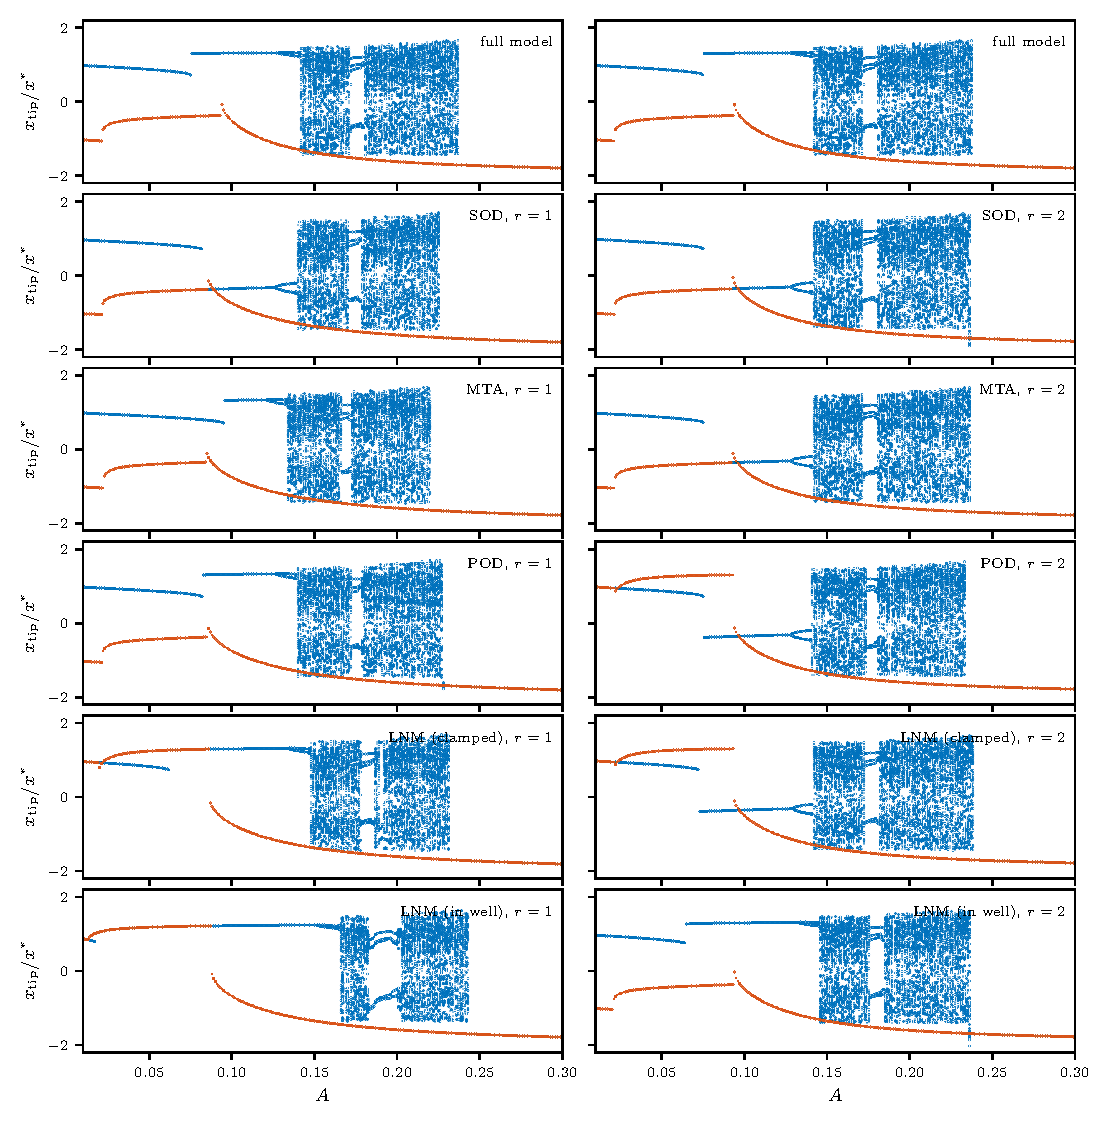
\includegraphics[width=\textwidth]{fig_mb_amp.pdf}
\caption{Two-well beam (S5) at $\varOmega=0.85\,\omega_{\mathrm w}$: amplitude bifurcation diagrams over the whole range swept. Tip displacement sampled once per forcing period, divided by $x^*$; up sweep blue, down sweep orange. Top: full model. Below: ROMs with $r=1$ (left) and $r=2$ (right). Some ROMs settle on the mirror orbit in the other well after the jump near $A=0.075$.}
\label{fig:mbamp}
\end{figure}

\begin{figure}[tbp]
\centering
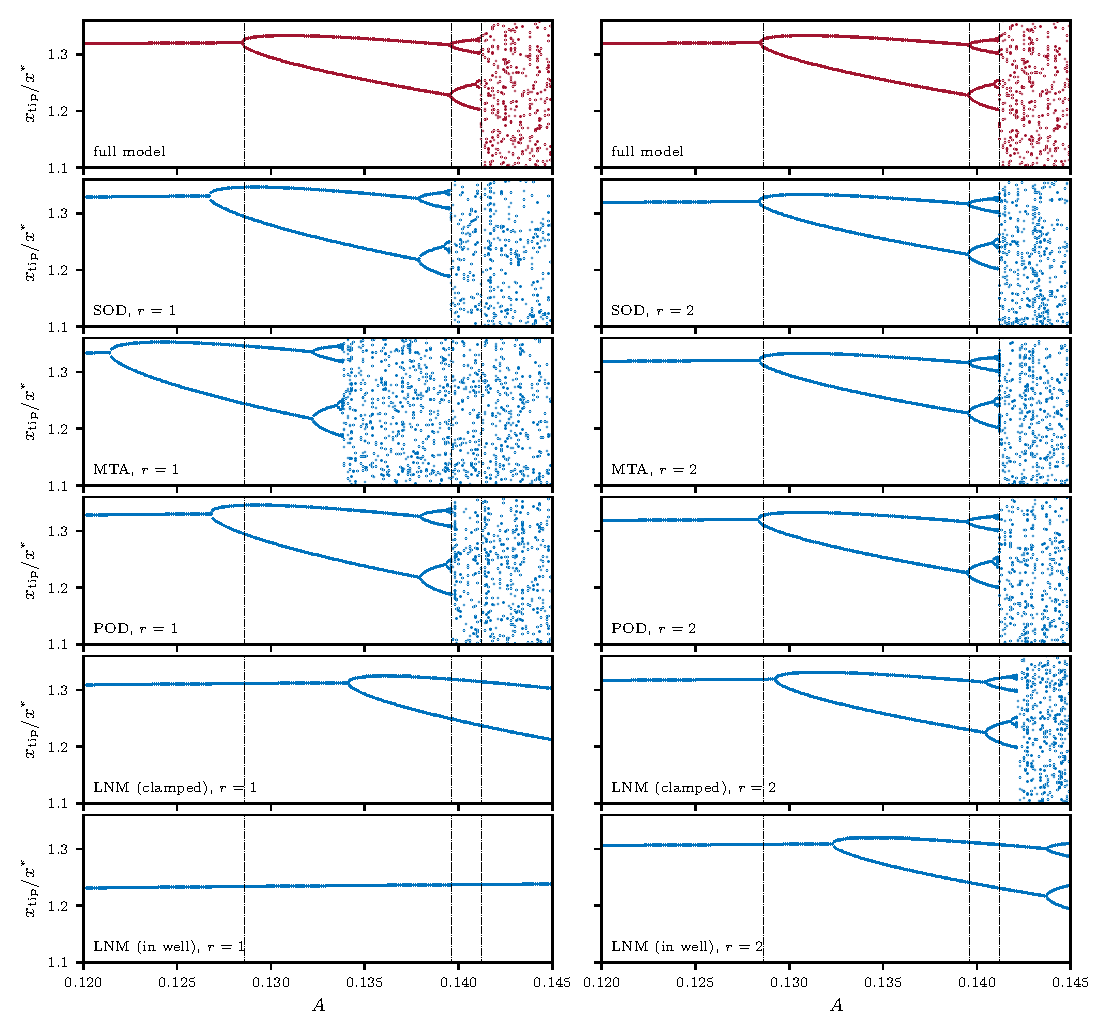
\includegraphics[width=\textwidth]{fig_mb_cascade.pdf}
\caption{The period-doubling cascade of Figure~\ref{fig:mbamp}, up sweep in steps of $10^{-4}$. ROMs on the mirror orbit are shown through it. Dotted: full-model onsets of period 2 and period 4, and the escape to cross-well motion. Left $r=1$, right $r=2$. The cascade of the in-well LNM ROM at $r=1$ lies above $A=0.15$.}
\label{fig:mbcasc}
\end{figure}

\paragraph{What the two-well beam adds.} The decay alone gave SOD the static correction at the nonlinear force. No location was supplied. In the amplitude sweep at one mode, SOD and POD placed the cascade best. They nearly coincide there, because one direction dominates a cross-well decay. With more modes, the model-based MTA basis was again best, as on S4 and on the linear benchmarks. At $r=3$ and 4 SOD followed within a factor of 7 (amplitude sweep) and 2 (frequency sweep). POD fell behind both.
\section{Computation cost}\label{sec:cost}
Are SOD ROMs faster, as reported \citep{Ilbeigi2018}, and if so, is the gain a property of SOD?
Two facts frame the answer.
A full-rank change of coordinates is a congruence of $(\bM,\bK)$ and a similarity of the first-order state matrix $\bm{A}$, so it leaves every eigenvalue unchanged.
An explicit integrator is limited by the spectral radius $\rho(\bm{A})$, not only by the highest natural frequency $\omega_{\max}$. With $\bC=\alpha\bM+\beta\bK$ the high finite-element modes are overdamped, and their real eigenvalues, about $\beta\omega^2$, can exceed $\omega_{\max}$. A change of coordinates leaves $\rho(\bm{A})$ unchanged; truncation can lower it.
What a change of coordinates can alter is how an adaptive integrator weighs its error estimate and, for an implicit integrator, how well its Newton iterations are conditioned.

\paragraph{Protocol.} Each model was integrated over 20 (S1) or 10 (S2) periods of mode 1 under a chirp load from $0.5\omega_1$ to $\omega_{\mathrm c}$, with light damping. The SOD and POD bases come from one random record (seed 5).
Every ROM was integrated in Ritz coordinates of its subspace: the eigenvectors of the reduced pencil $(\bm{\varPhi}^{\mathsf T}\bK\bm{\varPhi},\bm{\varPhi}^{\mathsf T}\bM\bm{\varPhi})$, normalized so that the reduced mass is the identity. Under Rayleigh damping the reduced stiffness and damping are then diagonal. The raw smooth modes, with unit Euclidean columns, are kept for one contrast.
Three integrators were used: RK45, the adaptive explicit Runge--Kutta pair of \citet{Dormand1980}; Radau, the implicit fifth-order Radau IIA method \citep{Hairer1996} with analytic Jacobian, both as implemented in SciPy \citep{Virtanen2020}; and central differences at 0.9 of $2/\omega_{\max}$. The central-difference scheme treats damping implicitly, $(\bM/\Delta t^2+\bC/(2\Delta t))\bx_{k+1}=\dots$, so its step limit is $2/\omega_{\max}$ whatever the damping.
Cost is compared at matched accuracy. For each model and adaptive integrator, the relative tolerance was swept from $10^{-3}$ to $10^{-9}$ in half decades. Two absolute tolerances were tried at each: one scalar, scaled to the physical response, and one per coordinate, scaled to that coordinate's largest value. The model is charged the run with the fewest function evaluations whose displacement error, against a tight reference of the same model, is at most $10^{-6}$. That run was then timed, best of three, single-threaded. The stiff full cantilever under RK45 is stability-limited at every tolerance and was run once.
All wall times in this paper were measured on one machine: a two-core Intel Xeon at 2.1\,GHz under Linux, with Python 3.13, NumPy 2.5 and SciPy 1.18, on one BLAS thread. The conclusions rest on evaluation and step counts, which do not depend on the machine.

\begin{table}[t]
\centering\small
\caption{Integration cost at matched accuracy: the least work to reach a displacement error of $10^{-6}$; light Rayleigh damping, chirp load. ROMs in Ritz coordinates of their subspace; ``raw'' is the same SOD subspace in unit-Euclidean smooth modes. $\rho(\bm{A}_r)$: spectral radius of the first-order state matrix. CD: central-difference steps at 0.9 of $2/\omega_{\max}$. LU: Radau matrix factorizations. --: the single stability-limited RK45 run did not reach $10^{-6}$. Script: \texttt{c36\_cost\_matched.py}, table \texttt{mktab\_c\_cost.py}.}
\label{tab:cost}
\resizebox{\textwidth}{!}{\begin{tabular}{llrrrrrrrr}
\toprule
system & model & $\omega_{\max}$ & $\rho(\bm{A}_r)$ & CD steps & RK45 evals & RK45 (s) & Radau evals & Radau LU & Radau (s)\\
\midrule
S1 & full, physical & 36.2 & 36.2 & 924 & 13\,562 & 0.23 & 13\,342 & 244 & 0.47\\
 & full, LNM coordinates & 36.2 & 36.2 & 924 & 12\,020 & 0.15 & 14\,729 & 212 & 0.39\\
 & LNM $r=4$ & 17.1 & 17.1 & 436 & 10\,922 & 0.14 & 15\,406 & 36 & 0.40\\
 & MTA $r=4$ & 18.9 & 18.9 & 483 & 12\,056 & 0.20 & 12\,967 & 448 & 0.40\\
 & POD $r=4$ & 17.1 & 17.1 & 436 & 10\,970 & 0.14 & 15\,559 & 40 & 0.47\\
 & SOD $r=4$ & 17.7 & 17.7 & 453 & 11\,540 & 0.15 & 15\,497 & 36 & 0.49\\
 & LNM $r=8$ & 30.6 & 30.6 & 780 & 12\,770 & 0.17 & 15\,236 & 222 & 0.45\\
 & MTA $r=8$ & 32.5 & 32.5 & 828 & 11\,168 & 0.19 & 14\,204 & 96 & 0.50\\
 & POD $r=8$ & 32.4 & 32.4 & 827 & 11\,168 & 0.14 & 14\,140 & 84 & 0.49\\
 & SOD $r=8$ & 32.9 & 32.9 & 838 & 11\,150 & 0.19 & 15\,169 & 228 & 0.44\\
 & SOD $r=8$, raw smooth modes & 32.9 & 32.9 & 838 & 13\,592 & 0.23 & 14\,353 & 124 & 0.37\\
\midrule
S2 & full, physical & $5.4\times10^{4}$ & $9.3\times10^{5}$ & 535\,013 & 35\,062\,052 & 471.22 & 62\,792 & 1\,760 & 3.19\\
 & full, LNM coordinates & $5.4\times10^{4}$ & $9.3\times10^{5}$ & 535\,013 & -- & -- & 58\,946 & 3\,350 & 4.00\\
 & LNM $r=4$ & 121 & 121 & 1\,201 & 40\,214 & 0.58 & 55\,920 & 3\,842 & 1.89\\
 & MTA $r=4$ & 135 & 135 & 1\,338 & 36\,002 & 0.40 & 62\,596 & 2\,922 & 1.99\\
 & POD $r=4$ & 121 & 121 & 1\,204 & 40\,790 & 0.61 & 56\,426 & 3\,920 & 1.92\\
 & SOD $r=4$ & 169 & 169 & 1\,679 & 44\,990 & 0.51 & 57\,876 & 52 & 1.74\\
 & LNM $r=8$ & 555 & 555 & 5\,514 & 53\,636 & 0.67 & 57\,290 & 3\,394 & 1.70\\
 & MTA $r=8$ & 717 & 717 & 7\,124 & 59\,834 & 0.85 & 57\,093 & 3\,316 & 2.02\\
 & POD $r=8$ & 882 & 882 & 8\,755 & 72\,416 & 0.77 & 57\,182 & 3\,346 & 1.68\\
 & SOD $r=8$ & 882 & 882 & 8\,755 & 72\,386 & 0.90 & 57\,151 & 3\,344 & 1.50\\
 & SOD $r=8$, raw smooth modes & 882 & 882 & 8\,755 & 71\,378 & 0.86 & 110\,084 & 6\,792 & 3.20\\
\bottomrule
\end{tabular}
% times: two-core Linux workspace, 14 Nov 2026
}
\end{table}

\begin{itemize}
\item \emph{Truncation sets the cost.} On S2 the full model is limited by its largest eigenvalue, real and equal to $-9.3\times10^5$: an overdamped finite-element mode under the $\beta\bK$ term, 17 times $\omega_{\max}$. RK45 needed $3.5\times10^7$ evaluations to reach $10^{-6}$; the four-mode LNM ROM needed $4.0\times10^4$, about 870 times fewer. Central-difference steps fell from 535\,013 to 1\,201. Radau is not stability-limited: it needed $6.3\times10^4$ evaluations for the full model and $5.6$--$6.3\times10^4$ for every ROM in Ritz coordinates.
\item \emph{Coordinates do not, at matched accuracy.} The order-8 SOD subspace of S2 needed 72\,386 RK45 evaluations in Ritz coordinates and 71\,378 in raw smooth modes; on S1 the raw basis needed 1.2 times as many. For Radau the raw smooth modes needed 1.9 times the evaluations and 2.0 times the factorizations of Ritz coordinates on S2. Their reduced mass matrix has condition number $7.4\times10^6$; in Ritz coordinates it is the identity. The full model needed 58\,946 Radau evaluations in LNM coordinates and 62\,792 in physical ones.
\item \emph{A fixed tolerance misleads.} At one fixed setting (relative tolerance $10^{-6}$, absolute $10^{-9}$), the order-8 SOD subspace of S2 needed 416\,k RK45 evaluations in raw smooth modes and 158\,k in Ritz coordinates, but the two runs reached errors of $2.1\times10^{-10}$ and $3.8\times10^{-9}$. At that setting Radau took 11.3\,s for the full model and 3.8\,s in LNM coordinates, at errors of $1.5\times10^{-8}$ and $4.8\times10^{-8}$ (\texttt{k1\_basis\_cost.py}, \texttt{k2\_matched\_cost.py}). An absolute tolerance weighs coordinates by their scale, and a change of coordinates changes the scale.
\item \emph{The SOD subspace is slightly stiffer.} The quasi-static direction raises the projected $\omega_{\max}$: 169 against 121 at $r=4$, and 882 against 555 at $r=8$, where SOD and POD span one subspace. At $10^{-6}$ the order-8 SOD ROM needed 1.35 times the RK45 evaluations of the LNM ROM. At $10^{-8}$, where accuracy limits the step, it needed 0.94 times as many (131\,684 against 139\,832). Radau cost the same for both.
\item \emph{Load bandwidth.} On S1 the chirp reaches $\omega_{\mathrm c}=23$, close to $\omega_{\max}=36.2$. Accuracy, not stability, then limits the step, and every model, the full one included, cost the same within 25\,\% (Table~\ref{tab:cost}).
\end{itemize}
\citet{Ilbeigi2018} studied a ten-dimensional, full-order SOD model of a nonlinear control system and reported that it ran about twice as fast as the original. A full-rank linear change of coordinates cannot change the eigenvalues. At a fixed tolerance, the coordinate scaling alone produced differences of that size here, and at matched accuracy they vanished. We have not tested their system.
For SOD ROMs we recommend Ritz coordinates of the retained subspace: they decouple the reduced model and, in every case tested, were no costlier than any other basis of the same subspace.


\section{Discussion}\label{sec:disc}
The paper set out to test whether an SOD basis holds the directions its training record visits, and whether that explains its being better and worse than the LNMs at once.
The evidence supports the hypothesis on the linear benchmarks. Three findings point the same way.
First, the geometry: at high order the random-trained SOD subspace contains the static vector of the training load about 190 times better than the LNMs, and that of the unseen load no better. Seven of its eight directions coincide with MTA built on the training load alone.
Second, the transfer test: given the same load locations, SOD and MTA ROMs agreed within a factor of 3.4; with one location missing, both lost their gain.
Third, the ladder: the same quasi-static direction enters at $r=3$, displaces an in-band mode until all in-band modes are present, and the error ratio to the LNMs turns from a loss into a gain at that order: 6.5 times worse at $r=5$, 1.4 times better at $r=6$, where all five in-band modes are present. Recognising modes by frequency removed the loss.
A band-limited free decay, which contains no quasi-static response, gave a basis with no static correction and LNM-level errors, as the hypothesis requires.

SOD therefore delivers static correction from response records: at the same load locations its ROMs came within a factor of 3.4 of MTA. It needs no eigensolution of the model, but the Galerkin ROM still needs $\bM$, $\bC$ and $\bK$, and SOD needs response records at every load location of interest. These cost more to simulate than the static solves of MTA.
What SOD needs from the loads is their spatial pattern, not their amplitude or time history. A load $\bm{b}\,g(t)$ has the static vector $\bK^{-1}\bm{b}$ for any $g$, and the gain carried over to new random loads at the training input. By the same argument, loads at several points must vary independently in the training records: a record of one fixed combination carries only that combination's static vector. The gain also needs clean records: at 40\,dB the training noise set an error floor 11--300 times above the LNMs.
A local nonlinear force is different. It acts whenever the nonlinear spring deforms, a free decay included, so the record carries its static correction without its location being supplied. On the two-well beam one cross-well decay put the static correction at the nonlinear force into the first SOD direction, $0.7^\circ$ from $\bK^{-1}\bm{e}_{\mathrm{tip}}$, without that location being supplied. The one-mode ROM then balanced the buckled equilibrium against the well frequency better than the three model-based vectors tested: the static vector and the clamped and in-well LNMs. On the COST F3 beam, decay-trained bases improved the backbone by two to three decades over the LNMs, as static correction did. The force keeps its location as the amplitude grows, so its static vector does not change either: the four-mode SOD ROM matched the backbone to about $10^{-6}$ up to 0.048\,J, about three times the energy of its training decay.

With complex modes the state-SOD planes likewise follow the record: a decay tilts them toward the modes it excites above the retained band, and a forced record by its quasi-static response (Section~\ref{sec:ic}). State-space SOD of a band-limited decay gave ROMs within a factor of 2.7 of complex-mode truncation on forced tests at state dimension 8. Its price is accelerations. Of the decays tested, those with little energy above the retained band, relative to the energy inside it, gave the most accurate ROMs. This is the rule an experimentalist applies in choosing a hammer tip.

In our tests the speed of SOD ROMs came from truncation, not from the SOD coordinates. A change of coordinates is a similarity of the state matrix, so it cannot move a stability limit. At matched accuracy it did not change the explicit cost either. Apparent speed-ups at a fixed tolerance come from how an absolute tolerance weighs coordinates of different scale. For implicit integration the coordinates matter through conditioning: on the stiff cantilever the raw smooth modes, whose reduced mass matrix is ill-conditioned, needed about twice the work of Ritz coordinates.

This is a simulation study, and what the evidence does not show is the same mechanism on measured records. The geometric test is direct here because every static vector is known. On a structure it would need the load locations and a model-free check of containment, such as the static deflection under a known load measured at the same sensors.

\paragraph{Limitations.} All data are simulated; noise enters only in the training-record test. Two nonlinear benchmarks have one local nonlinearity each, fixed in location; a distributed nonlinearity, whose force pattern changes with amplitude, was not tested. The geometric tests use one benchmark (S2, light damping, 20 realizations). We tested linear Galerkin bases only, with no manifold-based ROM \citep{Haller2016,Jain2017} for comparison. Cost was measured with two integrators of one library on one machine, against displacement error over one chirp load.

\section{Conclusions}\label{sec:concl}
An SOD basis contains the directions its training record visits. Under forcing that is the static correction at the load locations the record saw, which MTA supplies from the model; with the same load locations the two bases performed within a factor of 3.4, and with one location missing both lost their gain. The basis is worse than the LNMs at low order because SOD ranks that same quasi-static direction by smoothness, and it displaces an in-band mode. Recognising modes by their own frequency, or by circularity in state-space SOD, and placing them first removes the loss. In the cost tests, speed came from truncation: at matched accuracy the coordinates of a subspace changed the explicit cost by at most 1.2 times, and Ritz coordinates halved the implicit cost of the raw smooth modes.
What the basis needs from the loads is therefore where they act, not their amplitude or time history. For external loads that means a training record at every load location. A local nonlinear force acts in a free decay, so one decay supplies its static correction without its location being known. This is where a data basis supplies what MTA cannot without the location: on the two-well beam, the first SOD direction of one decay lay $0.7^\circ$ from the static vector at the nonlinear spring.


\appendix
\section{Proofs}\label{app:proofs}

\paragraph{Configuration SOD.} Let $\bx=\bPhi\bm{\eta}$, with $\bPhi$ the mass-normalized LNMs, and assume full-rank data. Then $\bSig_x=\bPhi\bm{G}_x\bPhi^{\mathsf T}$ and $\bSig_v=\bPhi\bm{G}_v\bPhi^{\mathsf T}$. Put $\bpsi=\bPhi^{-\mathsf T}\bm{\chi}$. The pencil $\bSig_v\bpsi=\mu\bSig_x\bpsi$ becomes
\begin{equation}
\bm{G}_v\bm{\chi}=\mu\,\bm{G}_x\bm{\chi},\qquad \bphi=\bSig_x\bpsi=\bPhi\bm{G}_x\bm{\chi} .
\label{eq:app_modal}
\end{equation}
\begin{itemize}
\item \emph{Sufficiency.} If $\bm{G}_x$ and $\bm{G}_v$ are diagonal, $\bm{\chi}_i\propto\bm{e}_i$. Then $\bphi_i\propto\bPhi\bm{e}_i$, the $i$th LNM, and $\mu_i=(\bm{G}_v)_{ii}/(\bm{G}_x)_{ii}$.
\item \emph{Necessity.} Let every $\bphi_i$ be an LNM and the $\mu_i$ distinct. Then $\bm{G}_x\bm{\chi}_i\propto\bm{e}_i$, so $\bm{\chi}_i\propto\bm{G}_x^{-1}\bm{e}_i$. The $\bm{\chi}_i$ are $\bm{G}_x$-orthogonal, hence $\bm{e}_i^{\mathsf T}\bm{G}_x^{-1}\bm{e}_j=0$ for $i\ne j$. So $\bm{G}_x^{-1}$, and with it $\bm{G}_x$, is diagonal. Then $\bm{\chi}_i\propto\bm{e}_i$, and \eqref{eq:app_modal} makes $\bm{G}_v$ diagonal.
\item \emph{Frequencies.} With both diagonal, $\mu_i=\omega_i^2$ if and only if $(\bm{G}_v)_{ii}=\omega_i^2(\bm{G}_x)_{ii}$. Write $(\bm{G}_v)_{ii}=\omega_i^2(1+\delta_i)(\bm{G}_x)_{ii}$. Then $\sqrt{\mu_i}=\omega_i(1+\delta_i)^{1/2}=\omega_i(1+\delta_i/2+O(\delta_i^2))$, and the mode is unchanged.
\item \emph{Correlation.} Let the off-diagonal entries of $\bm{G}_x$ and $\bm{G}_v$ be of order $\epsilon$. Standard perturbation of \eqref{eq:app_modal} gives $\bm{\chi}_i=\bm{e}_i+\sum_{j\ne i}c_{ij}\bm{e}_j+O(\epsilon^2)$. Here $c_{ij}=[(\bm{G}_v)_{ji}-\mu_i(\bm{G}_x)_{ji}]/[(\mu_i-\mu_j)(\bm{G}_x)_{jj}]$. The mode rotates at first order; $\mu_i$ changes at second order.
\end{itemize}

\paragraph{Defect of a damped decay.} Take $\ddot\eta+2\zeta\omega\dot\eta+\omega^2\eta=0$ with $\eta(0)=\hat\eta\cos\varphi$, $\dot\eta(0)=-\omega\hat\eta\sin\varphi$, and $0<\zeta<1$. Let $I_x=\int_0^\infty\eta^2\,\mathrm{d}t$ and $I_v=\int_0^\infty\dot\eta^2\,\mathrm{d}t$. Multiply the equation by $\dot\eta$ and integrate; then multiply by $\eta$ and integrate. The boundary terms give
\begin{equation}
I_v=\frac{\omega\hat\eta^2}{4\zeta},\qquad
\omega^2 I_x=I_v\left(1+4\zeta^2\cos^2\varphi-2\zeta\sin2\varphi\right).
\end{equation}
Thus $\mu=I_v/I_x=\omega^2/(1+4\zeta^2\cos^2\varphi-2\zeta\sin2\varphi)$. Released from rest ($\varphi=0$), $\mu=\omega^2/(1+4\zeta^2)$: the defect is $-4\zeta^2/(1+4\zeta^2)$, second order in $\zeta$. With an initial velocity the first-order term $-2\zeta\sin2\varphi$ appears; it averages to zero over $\varphi$. The infinite horizon stands for a record that has decayed.

\paragraph{Proposition~\ref{prop:ssod}.} Consider a free response, $\dot{\bm{y}}=\bm{A}\bm{y}$. In real modal coordinates $\bm{y}=\bm{P}\bm{\xi}$, $\dot{\bm{\xi}}=\bm{L}\bm{\xi}$ with $\bm{L}=\operatorname{blockdiag}(\bm{L}_i)$. Assume $\bm{P}$ invertible and $\avg{\bm{\xi}\bm{\xi}^{\mathsf T}}=\bm{G}=\operatorname{blockdiag}(\bm{G}_i)$ with each $\bm{G}_i\succ0$. Then $\avg{\bm{y}\bm{y}^{\mathsf T}}=\bm{P}\bm{G}\bm{P}^{\mathsf T}$ and $\avg{\dot{\bm{y}}\dot{\bm{y}}^{\mathsf T}}=\bm{P}\bm{L}\bm{G}\bm{L}^{\mathsf T}\bm{P}^{\mathsf T}$. With $\bpsi=\bm{P}^{-\mathsf T}\bm{\chi}$, the pencil \eqref{eq:ssod} becomes
\begin{equation}
\bm{L}\bm{G}\bm{L}^{\mathsf T}\bm{\chi}=\mu\,\bm{G}\bm{\chi} .
\end{equation}
Both sides are block diagonal, so the pencil splits into $2\times2$ pencils $\bm{L}_i\bm{G}_i\bm{L}_i^{\mathsf T}\bm{\chi}=\mu\bm{G}_i\bm{\chi}$.
\begin{itemize}
\item \emph{Pair product.} $\mu_{i,a}\mu_{i,b}=\det(\bm{L}_i\bm{G}_i\bm{L}_i^{\mathsf T})/\det\bm{G}_i=(\det\bm{L}_i)^2=|s_i|^4$.
\item \emph{Span.} An eigenvector $\bm{\chi}$ of plane $i$ is zero outside that block. Its smooth mode $\bphi=\bm{P}\bm{G}\bm{\chi}$ lies in the span of $\bm{P}_i=(\operatorname{Re}\,\bm{v}_i,\operatorname{Im}\,\bm{v}_i)$.
\item \emph{Equal values.} Write $\bm{L}_i=\sigma_i\bm{I}+\omega_i\bm{J}$ with $\bm{J}=\big[\begin{smallmatrix}0&1\\-1&0\end{smallmatrix}\big]$, and $\bm{S}=\bm{G}_i^{1/2}$. The two values are equal if and only if $\bm{D}\bm{D}^{\mathsf T}=\mu\bm{I}$, where $\bm{D}=\bm{S}^{-1}\bm{L}_i\bm{S}=\sigma_i\bm{I}+\omega_i\bm{N}$ and $\bm{N}=\bm{S}^{-1}\bm{J}\bm{S}$. If $\bm{G}_i\propto\bm{I}$, then $\bm{N}=\bm{J}$ and $\bm{D}\bm{D}^{\mathsf T}=|s_i|^2\bm{I}$. Conversely, a real $2\times2$ matrix with $\bm{D}\bm{D}^{\mathsf T}\propto\bm{I}$ and $\det\bm{D}>0$ is a scaled rotation, $\gamma_1\bm{I}+\gamma_2\bm{J}$. Since $\operatorname{tr}\,\bm{N}=0$ and $\det\bm{N}=1$, this forces $\bm{N}=\pm\bm{J}$, that is $\bm{J}\bm{S}=\pm\bm{S}\bm{J}$. A symmetric $\bm{S}$ commutes with $\bm{J}$ only if $\bm{S}\propto\bm{I}$. It anticommutes only if $\operatorname{tr}\,\bm{S}=0$, which $\bm{S}\succ0$ excludes. Hence $\bm{G}_i\propto\bm{I}$.
\end{itemize}
For an undamped mode, $\bm{L}_i=\omega_i\bm{J}$ and $\bm{G}_i\propto\bm{I}$ is the modal virial balance. The pair product needs only the decorrelation of the planes.

\section{Code and data}\label{app:repro}
All results are simulations in Python (NumPy, SciPy, Matplotlib). The scripts, their stored outputs, the reproduction manual and a driver that reruns them will be made public on submission, archived at Zenodo \url{https://doi.org/10.5281/zenodo.24248585} and developed at \url{https://github.com/nld-uri/sod-static-correction}.
The SOD computations use the SOD Toolbox, released with the scripts (\url{https://github.com/nld-uri/sod-toolbox}).
It provides configuration and state SOD, the recognition rules of Section~\ref{sec:recog}, and the bases and ROMs compared here, in Python and base MATLAB.
Its tests check it against the code that produced the stored outputs. Rerunning the recognition, mode-shape and nonlinear scripts on it changed no printed number.
The geometric measures of Sections~\ref{sec:adds} and \ref{sec:displace} come from \texttt{g1\_static\_containment.py}, \texttt{g2\_mode\_displacement.py} and \texttt{g3\_third\_direction.py}; the costs of Section~\ref{sec:cost} from \texttt{c36\_cost\_matched.py}, \texttt{k1\_basis\_cost.py} and \texttt{k2\_matched\_cost.py}. Each reuses the seeds and draw order of the ensemble script it complements.
A reproduction manual maps every section, table, figure and quoted number to its script and random seed. It also gives the output file and run time. Each script is deterministic for its seed.

\section*{CRediT authorship contribution statement}
\textbf{D.~Chelidze:} Conceptualization, Methodology, Software, Formal analysis, Investigation, Visualization, Writing -- original draft, Writing -- review \& editing, Supervision, Funding acquisition.

\section*{Declaration of competing interest}
The author declares that he has no known competing financial interests or personal relationships that could have appeared to influence the work reported in this paper.

\section*{Funding}
The author kindly acknowledges the indirect financial support provided by the National Institute for Undersea Vehicle Technology (NIUVT) and the Office of Naval Research (ONR) under grant number N00014-24-1-2093.

\section*{Data availability}
Every number, table and figure in this paper is produced from the models alone by the Python scripts named in Appendix~\ref{app:repro}; there are no measured data. The scripts, their stored outputs and the reproduction manual will be made public on submission, archived at Zenodo \url{https://doi.org/10.5281/zenodo.24248585}. The SOD computations use the SOD Toolbox (\url{https://github.com/nld-uri/sod-toolbox}).

\section*{Declaration of generative AI and AI-assisted technologies in the manuscript preparation process}
During the preparation of this work the author used Claude (Anthropic; Claude Opus 5 and Claude Opus 5.5) accessed through the Claude Science research environment and Claude Code, in order to write and debug the simulation, analysis and figure code, to design and run the numerical experiments reported here, to carry out the literature searches from which parts of the reference list were selected and to check the cited sources against the text, and to draft, edit and restructure the manuscript text. After using these tools the author reviewed and edited the content as needed. The reported results can be regenerated with the scripts and reproduction manual described in Appendix~\ref{app:repro}, and the bibliographic details of the cited references were checked against Crossref and OpenAlex and by the author. The author takes full responsibility for the content of the published article.

\bibliographystyle{elsarticle-num-names}
\bibliography{../refs}
\end{document}
